\documentclass[11pt,a4paper]{article}
\usepackage[margin=2.5cm]{geometry}
\usepackage{iohk}
\usepackage{microtype}
\usepackage{mathpazo} % nice fonts
\usepackage{amsmath}
\usepackage{amssymb}
\usepackage{latexsym}
\usepackage{mathtools}
\usepackage{stmaryrd}
\usepackage{extarrows}
\usepackage{slashed}
\usepackage[colon]{natbib}
\usepackage[unicode=true,pdftex,pdfa,colorlinks=true]{hyperref}
\usepackage{xcolor}
\usepackage[capitalise,noabbrev,nameinlink]{cleveref}
\usepackage{float}
\floatstyle{boxed}
\restylefloat{figure}
\usepackage{listings} % for code blocks.
%%
%% Package `semantic` can be used for writing inference rules.
%%
\usepackage{semantic}
%% Setup for the semantic package
\setpremisesspace{20pt}
\usepackage{tikz}
\usetikzlibrary{decorations.pathreplacing, positioning, arrows.meta, calc}

%%
%% Types
%%
\newcommand{\Bool}{\type{Bool}}
\newcommand{\Tx}{\type{Tx}}
\newcommand{\Ix}{\type{Ix}}
\newcommand{\TxId}{\type{TxId}}
\newcommand{\Addr}{\type{Addr}}
\newcommand{\UTxO}{\type{UTxO}}
\newcommand{\Value}{\type{Value}}
\newcommand{\Lovelace}{\type{Lovelace}}
\newcommand{\PrtclConsts}{\type{PrtclConsts}}
%% Adding witnesses
\newcommand{\TxIn}{\type{TxIn}}
\newcommand{\TxOut}{\type{TxOut}}
\newcommand{\VKey}{\type{VKey}}
\newcommand{\SKey}{\type{SKey}}
\newcommand{\Hash}{\type{Hash}}
\newcommand{\SkVk}{\type{SkVk}}
\newcommand{\Sig}{\type{Sig}}
\newcommand{\Data}{\type{Data}}
%% Adding delegation
\newcommand{\Epoch}{\type{Epoch}}
\newcommand{\VKeyGen}{\type{VKeyGen}}
%% Blockchain
\newcommand{\Gkeys}{\var{G_{keys}}}
\newcommand{\Block}{\type{Block}}
\newcommand{\CEEnv}{\type{CEEnv}}
\newcommand{\CEState}{\type{CEState}}
\newcommand{\BDEnv}{\type{BDEnv}}
\newcommand{\BDState}{\type{BDState}}
\newcommand{\Slot}{\type{Slot}}
\newcommand{\SlotCount}{\type{SlotCount}}

%%
%% Functions
%%
\newcommand{\txins}[1]{\fun{txins}~ \var{#1}}
\newcommand{\txid}[1]{\fun{txid}~ \var{#1}}
\newcommand{\txouts}[1]{\fun{txouts}~ \var{#1}}
\newcommand{\values}[1]{\fun{values}~ #1}
\newcommand{\balance}[1]{\fun{balance}~ \var{#1}}
%% UTxO witnesses
\newcommand{\inputs}[1]{\fun{inputs}~ \var{#1}}
\newcommand{\wits}[1]{\fun{wits}~ \var{#1}}
\newcommand{\verify}[3]{\fun{verify} ~ #1 ~ #2 ~ #3}
\newcommand{\sign}[2]{\fun{sign} ~ #1 ~ #2}
\newcommand{\serialised}[1]{\llbracket \var{#1} \rrbracket}
\newcommand{\addr}[1]{\fun{addr}~ \var{#1}}
\newcommand{\hash}[1]{\fun{hash}~ \var{#1}}
\newcommand{\txbody}[1]{\fun{txbody}~ \var{#1}}
\newcommand{\txfee}[1]{\fun{txfee}~ \var{#1}}
\newcommand{\minfee}[2]{\fun{minfee}~ \var{#1}~ \var{#2}}
% wildcard parameter
\newcommand{\wcard}[0]{\underline{\phantom{a}}}
%% Adding ledgers...
\newcommand{\utxo}[1]{\fun{utxo}~ #1}
%% Delegation
\newcommand{\delegatesName}{\fun{delegates}}
\newcommand{\delegates}[3]{\delegatesName~#1~#2~#3}
\newcommand{\dwho}[1]{\fun{dwho}~\var{#1}}
\newcommand{\depoch}[1]{\fun{depoch}~\var{#1}}
%% Delegation witnesses
\newcommand{\dbody}[1]{\fun{dbody}~\var{#1}}
\newcommand{\dwit}[1]{\fun{dwit}~\var{#1}}
%% Blockchain
\newcommand{\bwit}[1]{\fun{bwit}~\var{#1}}
\newcommand{\bslot}[1]{\fun{bslot}~\var{#1}}
\newcommand{\bbody}[1]{\fun{bbody}~\var{#1}}
\newcommand{\bdlgs}[1]{\fun{bdlgs}~\var{#1}}

%\includeonly{update-mechanism, delegation, blockchain-interface}

%% Parameters that control floats placement. See https://robjhyndman.com/hyndsight/latex-floats/
\setcounter{topnumber}{2}
\setcounter{bottomnumber}{2}
\setcounter{totalnumber}{4}
\renewcommand{\topfraction}{0.85}
\renewcommand{\bottomfraction}{0.85}
\renewcommand{\textfraction}{0.15}
\renewcommand{\floatpagefraction}{0.7}

\begin{document}

\input{frontmatter.tex}

\tableofcontents
\listoffigures

\section{Introduction}
\label{sec:introduction}

This specification models the \textit{conditions} that the different parts of a
transaction have to fulfill so that they can extend a ledger, which is
represented here as a list of transactions. In particular, we model the
following aspects:

\begin{description}
\item[Preservation of value] relationship between the total value of input and
  outputs in a new transaction, and the unspent outputs.
\item[Witnesses] authentication of parts of the transaction data by means of
  cryptographic entities (such as signatures and private keys) contained in
  these transactions.
\item[Delegation] validity of delegation certificates, which delegate
  block-signing rights.
\item[Update validation] voting mechanism which captures the identification of
  the voters, and the participants that can post update proposals.
\end{description}

The following aspects will not be modeled (since they are not part of the Byron
release):
\begin{description}
\item[Stake] staking rights associated to an addresses.
\end{description}


\section{Notation}\label{sec:notation}

\begin{description}
\item[Natural Numbers] The set $\mathbb{N}$ refers to the set of all natural
  numbers $\{0, 1, 2, \ldots\}$.
\item[Powerset] Given a set $\type{X}$, $\powerset{\type{X}}$ is the set of all
  the subsets of $X$.
\item[Sequences] Given a set $\type{X}$, $\seqof{\type{X}}$ is the set of
  sequences having elements taken from $\type{X}$. The empty sequence is
  denoted by $\epsilon$, and given a sequence $\Lambda$, $\Lambda; \type{x}$ is
  the sequence that results from appending $\type{x} \in \type{X}$ to
  $\Lambda$.
\item[Functions] $A \to B$ denotes a \textbf{total function} from $A$ to $B$.
  Given a function $f$ we write $f~a$ for the application of $f$ to argument
  $a$.
\item[Fibre] Given a function $f: A \to B$ and $b\in B$, we write
  $f^{-1}~b$ for the \textbf{fibre} of $f$ at $b$, which is defined by
  $\{a \mid\ f~ a =  b\}$.
\item[Maps and partial functions] $A \mapsto B$ denotes a \textbf{partial
    function} from $A$ to $B$, which can be seen as a map (dictionary) with
  keys in $A$ and values in $B$. Given a map $m \in A \mapsto B$, notation
  $a \mapsto b \in m$ is equivalent to $m~ a = b$. Given a set $A$,
  $A \mapsto A$ represents the identity map on $A$:
  $\{a \mapsto a \mid a \in A\}$. The $\emptyset$ symbol is also used to
  represent the empty map as well.
\item[Domain and range operations] Given a relation
  $R \in \powerset{(A \times B)}$ we make use of the \textit{domain-restriction},
  \textit{domain-exclusion}, and \textit{range-restriction} operators, which
  are defined in \cref{fig:domain-and-range-ops}. Note that a map $A \mapsto B$
  can be seen as a relation, which means that these operators can be
  applied to maps as well.
\item[Integer ranges] Given $a, b \in \mathbb{R}$, $[a, b]$ denotes the
  sequence $[i \mid a \leq i \leq b]$ . Ranges can have open ends: $[.., b]$
  denotes sequence $[i \mid i \leq b]$, whereas $[a, ..]$ denotes sequence
  $[i \mid a \leq i]$. Furthermore, sometimes we use $[a, b]$ to denote a set
  instead of a sequence. The context in which it is used should provide enough
  information about the specific type.
\item[Domain and range operations on sequences] We overload the $\restrictdom$,
  $\subtractdom$, and $\restrictrange$ to operate over sequences. So for
  instance given $S \in \seqof{A}$, and $R \in \seqof{(A \times B)}$:
  $A \restrictdom R$ denotes the sequence
  $[ (a, b) \mid (a, b) \in R, a \in S]$.
\item[Wildcard variables] When a variable is not needed in a term, we replace
  it by $\wcard$ to make it explicit that we do not use this variable in the
  scope of the given term.
\item[Implicit existential quantifications] Given a predicate
  $P \in X \to Bool$, we use $P \wcard$ as a shorthand notation for
  $\exists x \cdot P~x$.
\end{description}

\begin{figure}[htb]
  \begin{align*}
    \var{S} \restrictdom \var{R}
    & = \{ (a, b) \mid (a, b) \in R, ~ a \in S \}
    & \text{domain restriction}
    \\
    S \subtractdom R
    & = \{ (a, b) \mid (a, b) \in R, ~ a \notin S \}
    & \text{domain exclusion}
    \\
    R \restrictrange S
    & = \{ (a, b) \mid (a, b) \in R, ~ b \in S \}
    & \text{range restriction}
  \end{align*}
  \caption{Domain and range operations}
  \label{fig:domain-and-range-ops}
\end{figure}

\section{Cryptographic primitives}
\label{sec:crypto-primitives}

Figure~\ref{fig:crypto-defs} introduces the cryptographic abstractions used in
this document. Note that we define a family of serialization functions
$\serialised{\wcard}_\type{A}$, for all types $\type{A}$ for which such
serialization function can be defined. When the context is clear, we omit the
type suffix, and use simply $\serialised{\wcard}$.

\begin{figure}[htb]
  \emph{Abstract types}
  %
  \begin{equation*}
    \begin{array}{r@{~\in~}lr}
      \var{vk} & \SKey & \text{signing key}\\
      \var{vk} & \VKey & \text{verifying key}\\
      \var{hk} & \Hash & \text{hash of a key}\\
      \sigma & \Sig  & \text{signature}\\
      \var{d} & \Data  & \text{data}\\
    \end{array}
  \end{equation*}
  \emph{Derived types}
  \begin{equation*}
    \begin{array}{r@{~\in~}lr}
      (sk, vk) & \SkVk & \text{signing-verifying key pairs}
    \end{array}
  \end{equation*}
  \emph{Abstract functions}
  %
  \begin{equation*}
    \begin{array}{r@{~\in~}lr}
      \hash{} & \VKey \to \Hash
      & \text{hash function} \\
      %
      \fun{verify} & \VKey \times \Data \times \Sig
      & \text{verification relation}\\
      \serialised{\wcard}_\type{A} & \type{A} \to \Data
      & \text{serialization function for values of type $\type{A}$}
    \end{array}
  \end{equation*}
  \emph{Constraints}
  \begin{align*}
    & \forall (sk, vk) \in \SkVk,~ m \in \Data,~ \sigma \in \Sig \cdot
      \verify{vk}{m}{\sigma} \iff \sign{sk}{m} = \sigma
  \end{align*}
  \emph{Notation}
  \begin{align*}
    & \mathcal{V}^\sigma_{\var{vk}}~{d} = \verify{vk}{d}{\sigma}
      & \text{shorthand notation for } \fun{verify}
  \end{align*}
  \caption{Cryptographic definitions}
  \label{fig:crypto-defs}
\end{figure}

\subsection{A note on serialization}
\label{sec:a-note-on-serialization}

\begin{definition}[Distributivity over serialization functions]
  For all types $\type{A}$ and $\type{B}$, given a function
  $\fun{f} \in \type{A} \to \type{B}$, we say that the serialization function
  for values of type $\type{A}$, namely $\serialised{ }_\type{A}$ distributes
  over $\fun{f}$ if there exists a function $\fun{f}_{\serialised{ }}$ such
  that for all $a \in \type{A}$:
  \begin{equation}
    \label{eq:distributivity-serialization}
    \serialised{\fun{f}~a}_\type{B} = \fun{f}_{\serialised{ }}~\serialised{a}_\type{A}
  \end{equation}
\end{definition}
The equality defined in \cref{eq:distributivity-serialization} means that the
following diagram commutes:

\[
  \begin{tikzcd}
    A \arrow{r}{\fun{f}} \arrow{d}{\serialised{ }_\type{A}}
    & B \arrow{d}{\serialised{ }_\type{B}} \\
    \Data \arrow{r}{\fun{f}_{\serialised{ }}} & \Data
  \end{tikzcd}
\]

Throughout this specification, whenever we use
$\serialised{\fun{f}~a}_\type{B}$, for some type $\type{B}$ and function
$\fun{f} \in \type{A} \to \type{B}$, we assume that $\serialised{ }_\type{A}$
distributes over $\fun{f}$ (see for example
Rule~\ref{eq:utxo-witness-inductive}). This property is what allow us to
extract a component of the serialized data (if it is available) without
deserializing it in the cases in which the deserialization function
($\serialised{\wcard}^{-1}_\type{A}$) doesn't behave as an inverse of
serialization:

\begin{equation*}
  \serialised{\wcard}^{-1}_\type{A} \cdot \serialised{\wcard}_\type{A} \neq \fun{id}_\type{A}
\end{equation*}

For the cases in which such an inverse exists, given a function $\fun{f}$, we
can readily define $\fun{f}_{\serialised{ }}$ as:

\begin{equation*}
  \fun{f}_{\serialised{ }} \dot{=} \serialised{\wcard}_\type{B}
                            . \fun{f}
                            . \serialised{\wcard}^{-1}_\type{A}
\end{equation*}


\include{serialisation}

\newcommand{\PPMMap}{\ensuremath{\type{Ppms}}}
\newcommand{\Lmax}{\ensuremath{\mathbb{L}_{\var{max}}}}
\section{UTxO}
\label{sec:state-trans-utxo-1}

The transition rules for unspent outputs are presented in
Figure~\ref{fig:rules:utxo}. The states of the UTxO transition system, along
with their types are defined in Figure~\ref{fig:defs:utxo}, here we define the
protocol parameters as an abstract type, this type is made concrete in
Section~\ref{sec:update}, where the update mechanism is discussed. Functions on
these types are defined in Figure~\ref{fig:derived-defs:utxo}. In particular,
note that in function $\fun{minfee}$ we make use of the fact that the
$\Lovelace$ type is an alias for the set of natural numbers ($\mathbb{N}$).

\begin{figure*}[htb]
  \emph{Abstract types}
  %
  \begin{equation*}
    \begin{array}{r@{~\in~}lr}
      \var{tx} & \Tx & \text{transaction}\\
      %
      \var{txid} & \TxId & \text{transaction id}\\
      %
      ix & \Ix & \text{transaction index}\\
      %
      \var{addr} & \Addr & \text{address}\\
      %
      \var{pps} & \PPMMap & \text{protocol parameters}
    \end{array}
  \end{equation*}
  \emph{Constants}
  %
  \begin{equation*}
    \begin{array}{r@{~=~}lr}
      \Lmax & 45*10^{15} & \text{Lovelace supply cap}\\
    \end{array}
  \end{equation*}
  \emph{Derived types}
  %
  \begin{equation*}
    \begin{array}{r@{~\in~}l@{\qquad=\qquad}r@{~\in~}lr}
      \ell & \Lovelace
      & n  & \{ n \mid n \in  \mathbb{N}, 0 \leq n \leq \Lmax \}
      & \text{currency value}
      \\
      \var{txin}
      & \TxIn
      & (\var{txid}, \var{ix})
      & \TxId \times \Ix
      & \text{transaction input}
      \\
      \var{txout}
      & \type{TxOut}
      & (\var{addr}, c)
      & \Addr \times \Lovelace
      & \text{transaction output}
      \\
      \var{utxo}
      & \UTxO
      & \var{txin} \mapsto \var{txout}
      & \TxIn \mapsto \TxOut
      & \text{unspent tx outputs}
    \end{array}
  \end{equation*}
  %
  \emph{Abstract Functions}
  \begin{equation*}
    \begin{array}{r@{~\in~}lr}
      \txid{} & \Tx \to \TxId & \text{compute transaction id}\\
      %
      \fun{txbody} & \Tx \to \powerset{\TxIn} \times (\Ix \mapsto \TxOut)
                                  & \text{transaction body}\\
      %
      \fun{txfee} & \Tx \to \Lovelace & \text{transaction fee}\\
      %
      \fun{a} & \PPMMap \to \mathbb{N} & \text{minumum fee factor}\\
      %
      \fun{b} & \PPMMap \to \mathbb{N} & \text{minumum fee constant}\\
      %
      \fun{txSize} & \Tx \to \mathbb{N} & \text{abstract size of a transaction}
    \end{array}
  \end{equation*}
  \caption{Definitions used in the UTxO transition system}
  \label{fig:defs:utxo}
\end{figure*}

\begin{figure}
  \begin{align*}
    & \fun{txins} \in \Tx \to \powerset{\TxIn}
    & \text{transaction inputs} \\
    & \txins{tx} = \var{inputs} \where \txbody{tx} = (\var{inputs}, ~\wcard)
    \nextdef
    & \fun{txouts} \in \Tx \to \UTxO
    & \text{transaction outputs as UTxO} \\
    & \fun{txouts} ~ \var{tx} =
      \left\{ (\fun{txid} ~ \var{tx}, \var{ix}) \mapsto \var{txout} ~
      \middle| \begin{array}{l@{~}c@{~}l}
                 (\_, \var{outputs}) & = & \txbody{tx} \\
                 \var{ix} \mapsto \var{txout} & \in & \var{outputs}
               \end{array}
      \right\}
    \nextdef
    & \fun{balance} \in \UTxO \to \mathbb{N}
    & \text{UTxO balance} \\
    & \fun{balance} ~ utxo = \sum_{(~\wcard ~ \mapsto (\wcard, ~c)) \in \var{utxo}} c\\
   \nextdef
   %
    & \fun{minfee} \in \PPMMap \to \Tx \to \mathbb{N} & \text{minimum fee}\\
    & \fun{minfee}~\var{pps}~\var{tx} =
      \fun{a}~\var{pps} * \fun{txSize}~\var{tx} + \fun{b}~\var{pps}
  \end{align*}
  \caption{Functions used in UTxO rules}
  \label{fig:derived-defs:utxo}
\end{figure}

\begin{figure}
  \emph{UTxO transitions}
  \begin{equation*}
    \_ \vdash
    \var{\_} \trans{utxo}{\_} \var{\_}
    \subseteq \powerset (\PPMMap \times \UTxO \times \Tx \times \UTxO)
  \end{equation*}
  \caption{UTxO transition-system types}
  \label{fig:ts-types:utxo}
\end{figure}

\begin{figure}
  \begin{equation}\label{eq:utxo-inductive}
    \inference
    { \txins{tx} \subseteq \dom \var{utxo} & \minfee{pps}{tx} \leq \txfee{tx}
      & \balance{(\txins{tx} \restrictdom \var{utxo})} \leq \Lmax \\
      \balance{(\txouts{tx})}  + \txfee{tx} =
      \balance{(\txins{tx} \restrictdom \var{utxo})}
    }
    {\var{pps} \vdash \var{utxo} \trans{utxo}{tx}
      (\txins{tx} \subtractdom \var{utxo}) \cup \txouts{tx}
    }
  \end{equation}
  \caption{UTxO inference rules}
  \label{fig:rules:utxo}
\end{figure}

Rule~\ref{eq:utxo-inductive} specifies under which conditions a transaction can
be applied to a set of unspent outputs, and how the set of unspent output
changes with a transaction:
\begin{itemize}
\item Each input spent in the transaction must be in the set of unspent
  outputs.
\item The transaction fee must be no less than the minimum fee, which depends
  on the transaction and the protocol parameters.
\item The balance of the unspent outputs in a transaction (i.e. the total
  amount paid in a transaction) plus the transaction fees must be equal to the
  amount of spent inputs, and these cannot exceed the $\Lovelace$ supply cap
  ($45*10^{15}$).
\item If the above conditions hold, then the new state will not have the inputs
  spent in transaction $\var{tx}$ and it will have the new outputs in
  $\var{tx}$.
\end{itemize}

\subsection{Properties}
\label{sec:utxo-properties}

\begin{todo}
  Can we prove properties of the transition system of this section? For
  instance we might like to formalize ``double spending'' and prove that these
  rules prevent it. Do we want it?
\end{todo}

\clearpage

\subsection{Witnesses}
\label{sec:witnesses}

The rules for witnesses are presented in Figure~\ref{fig:rules:utxow}.
The definitions used in Rule~\ref{eq:utxo-witness-inductive} are given in
Figure~\ref{fig:defs:utxow}. Note that
Rule~\ref{eq:utxo-witness-inductive} uses the transition relation defined in
Figure~\ref{fig:rules:utxo}. The main reason for doing this is to define
the rules incrementally, modeling different aspects in isolation to keep the
rules as simple as possible. Also note that the $\trans{utxo}{}$ relation could
have been defined in terms of $\trans{utxow}{}$ (thus composing the rules in a
different order). The choice here is arbitrary.

\begin{figure}[htb]
  \emph{Abstract functions}
  %
  \begin{equation*}
    \begin{array}{r@{~\in~}lr}
      \fun{wits} & \Tx \to \powerset{(\VKey \times \Sig)}
      & \text{witnesses of a transaction}\\
      \fun{hash_{spend}} & \Addr \mapsto \Hash
      & \text{hash of a spending key in an address}\\
    \end{array}
  \end{equation*}
  \caption{Definitions used in the UTxO transition system with witnesses}
  \label{fig:defs:utxow}
\end{figure}

\begin{figure}[htb]
  \begin{align*}
    & \addr{}{} \in \UTxO \to \TxIn \mapsto \Addr & \text{address of an input}\\
    & \addr{utxo} = \{ i \mapsto a \mid i \mapsto (a, \wcard) \in \var{utxo} \} \\
    \nextdef
    & \fun{addr_h} \in \UTxO \to \TxIn \mapsto \Hash & \text{hash of an input address}\\
    & \fun{addr_h}~utxo = \{ i \mapsto h \mid i \mapsto (a, \wcard) \in \var{utxo}
      \wedge a \mapsto h \in \fun{hash_{spend}} \}
  \end{align*}
  \caption{Functions used in rules witnesses}
  \label{fig:derived-defs:utxow}
\end{figure}

\begin{figure}
  \emph{UTxO with witness transitions}
  \begin{equation*}
    \var{\_} \vdash
    \var{\_} \trans{utxow}{\_} \var{\_}
    \subseteq \powerset (\PPMMap \times \UTxO \times \Tx \times \UTxO)
  \end{equation*}
  \caption{UTxO with witness transition-system types}
  \label{fig:ts-types:utxow}
\end{figure}

\begin{figure}
  \begin{equation}
    \label{eq:utxo-witness-inductive}
    \inference
    { \var{pps} \vdash \var{utxo} \trans{utxo}{tx} \var{utxo'}\\ ~ \\
      & \forall i \in \txins{tx} \cdot \exists (\var{vk}, \sigma) \in \wits{\var{tx}}
      \cdot
      \mathcal{V}^\sigma_{\var{vk}}~{\serialised{\txbody{tx}}}
      \wedge  \fun{addr_h}~{utxo}~i = \hash{vk}\\
    }
    {\var{pps} \vdash \var{utxo} \trans{utxow}{tx} \var{utxo'}}
  \end{equation}
  \caption{UTxO with witnesses inference rules}
  \label{fig:rules:utxow}
\end{figure}


\section{Delegation}
\label{sec:delegation}

\newcommand{\DSEnv}{\type{DSEnv}}
\newcommand{\DSState}{\type{DSState}}
\newcommand{\DCert}{\type{DCert}}
\newcommand{\DState}{\type{DState}}
\newcommand{\DEState}{\type{DEState}}

An agent owning a key that can sign new blocks can delegate its signing rights
to another key by means of \textit{delegation certificates}. These certificates
are included in the ledger, and therefore also included in the body of the
blocks in the blockchain.

There are several restrictions on a certificate posted on the blockchain:
\begin{enumerate}
\item Only genesis keys can delegate.
\item Certificates must be properly signed by the delegator.
\item Any given key can delegate at most once per-epoch.
\item Any given key can issue at most one certificate in a given slot.
\item The epochs in certificates cannot refer to past epochs. This mechanism
  prevents replay attacks.
\item Certificates do not become active immediately, but they require a certain
  number of slots till they become stable in all the nodes.
\end{enumerate}
These conditions are formalized in \cref{fig:rules:delegation-scheduling}.
Rule~\ref{eq:rule:delegation-scheduling} determines when a certificate can
become ``scheduled''. The definitions used in this rules are presented in
\cref{fig:defs:delegation-scheduling}, and the types of the system induced by
$\trans{sdeleg}{\wcard}$ are presented in
\cref{fig:ts-types:delegation-scheduling}.

\begin{figure}[htb]
  \emph{Abstract types}
  \begin{equation*}
    \begin{array}{r@{~\in~}lr}
      c & \DCert & \text{delegation certificate}\\
      \var{vk_g} & \VKeyGen & \text{genesis verification key}\\
    \end{array}
  \end{equation*}

  \emph{Derived types}
  \begin{equation*}
    \begin{array}{r@{~\in~}l@{\qquad=\qquad}r@{~\in~}lr}
      \var{e} & \Epoch & n & \mathbb{N} & \text{epoch}\\
      \var{s} & \Slot & s & \mathbb{N} & \text{slot}\\
      \var{d} & \SlotCount & s & \mathbb{N} & \text{slot}
    \end{array}
  \end{equation*}

  \emph{Constraints}
  \begin{align*}
    \VKeyGen \subseteq \VKey
  \end{align*}

  \emph{Abstract functions}
  \begin{equation*}
    \begin{array}{r@{~\in~}lr}
      \fun{dbody} & \DCert \to (\VKey \times \Epoch)
      & \text{body of the delegation certificate}\\
      \fun{dwit} & \DCert \to (\VKeyGen \times \Sig)
      & \text{witness for the delegation certificate}\\
      \fun{dwho} & \DCert \mapsto (\VKeyGen \times \VKey)
      & \text{who delegates to whom in the certificate}\\
      \fun{depoch} & \DCert \mapsto \Epoch
      & \text{certificate epoch}
    \end{array}
  \end{equation*}
  \caption{Delegation scheduling definitions}
  \label{fig:defs:delegation-scheduling}
\end{figure}

\begin{figure}[htb]
  \emph{Delegation scheduling environments}
  \begin{equation*}
    \DSEnv =
    \left(
      \begin{array}{r@{~\in~}lr}
        \mathcal{K} & \powerset{\VKeyGen} & \text{allowed delegators}\\
        \var{e} & \Epoch & \text{epoch}\\
        \var{s} & \Slot & \text{slot}\\
        \var{d} & \SlotCount & \text{certificate liveness parameter}
      \end{array}
    \right)
  \end{equation*}

  \emph{Delegation scheduling states}
  \begin{equation*}
    \DSState
    = \left(
      \begin{array}{r@{~\in~}lr}
        \var{sds} & \seqof{(\Slot \times (\VKeyGen \times \VKey))} & \text{scheduled delegations}\\
        \var{eks} & \powerset{(\Epoch \times \VKeyGen)} & \text{key-epoch delegations}
      \end{array}
    \right)
  \end{equation*}

  \emph{Delegation scheduling transitions}
  \begin{equation*}
    \var{\_} \vdash
    \var{\_} \trans{sdeleg}{\_} \var{\_}
    \subseteq \powerset (\DSEnv \times \DSState \times \DCert \times \DSState)
  \end{equation*}
  \caption{Delegation scheduling transition-system types}
  \label{fig:ts-types:delegation-scheduling}
\end{figure}

\begin{figure}[htb]
  \begin{equation}
    \label{eq:rule:delegation-scheduling}
    \inference
    {
      (\var{vk_s},~ \sigma) = \dwit{c}
      & \verify{vk_s}{\serialised{\dbody{c}}}{\sigma} & vk_s \in \mathcal{K}\\ ~ \\
      (\var{vk_s},~ \var{vk_d}) = \dwho{c} & e_d = \depoch{c}
      & (e_d,~ \var{vk_s}) \notin \var{eks} & e \leq e_d \\ ~ \\
      (s + d,~ (\var{vk_s},~ \wcard)) \notin \var{sds}\\
    }
    {
      {\begin{array}{l}
       \mathcal{K}\\
        e\\
        s\\
        d
      \end{array}}
      \vdash
      {
        \left(
          \begin{array}{l}
            \var{sds}\\
            \var{eks}
          \end{array}
        \right)
      }
      \trans{sdeleg}{c}
      {
        \left(
          \begin{array}{l}
            \var{sds}; (s + d,~ (\var{vk_s},~ \var{vk_d}))\\
            \var{eks} \cup \{(e_d,~ \var{vk_s})\}
          \end{array}
        \right)
      }
    }
  \end{equation}
  \caption{Delegation scheduling rules}
  \label{fig:rules:delegation-scheduling}
\end{figure}

Once a scheduled certificate becomes active
(see~\cref{sec:delegation-interface-rules}), the delegation map is changed by
it. \cref{fig:rules:delegation} models such change.

\begin{figure}[htb]
  \begin{align*}
    & \unionoverride \in (A \mapsto B) \to (A \mapsto B) \to (A \mapsto B)
    & \text{union override}\\
    & d_0 \unionoverride d_1 = d_1 \cup (\dom d_1 \subtractdom d_0)
  \end{align*}
  \caption{Functions used in delegation rules}
  \label{fig:funcs:delegation}
\end{figure}

\begin{figure}[htb]
  \emph{Delegation states}
  \begin{align*}
    & \DState
      = \left(
        \begin{array}{r@{~\in~}lr}
          \var{dms} & \VKeyGen \mapsto \VKey & \text{delegation map}\\
          \var{dws} & \VKeyGen \mapsto \Slot & \text{when last delegation occurred}\\
        \end{array}\right)
  \end{align*}
  \emph{Delegation transitions}
  \begin{equation*}
    \_ \vdash \_ \trans{adeleg}{\_} \_ \in
    \powerset (\DState \times (\Slot \times (\VKeyGen \times \VKey)) \times \DState)
    \end{equation*}
  \caption{Delegation transition-system types}
  \label{fig:ts-types:delegation}
\end{figure}

\begin{figure}[htb]
  \begin{equation}\label{eq:rule:delegation-change}
    \inference
    {\var{vk_s} \mapsto s_p \in \var{dws} \Rightarrow s_p < s
    }
    {
      \left(
      \begin{array}{r}
        \var{dms}\\
        \var{dws}
      \end{array}
      \right)
      \trans{adeleg}{(s,~ (vk_s,~ vk_d))}
      \left(
      \begin{array}{lcl}
        \var{dms} & \unionoverride & \{\var{vk_s} \mapsto \var{vk_d}\}\\
        \var{dws} & \unionoverride & \{\var{vk_s} \mapsto s \}
      \end{array}
      \right)
    }
  \end{equation}
  \nextdef
  \begin{equation}\label{eq:rule:delegation-nop}
    \inference
    {\var{vk_s} \mapsto s_p  \in \var{dws}  \wedge s \leq s_p
    }
    {
      \left(
      \begin{array}{r}
        \var{dms}\\
        \var{dws}
      \end{array}
      \right)
      \trans{adeleg}{(s,~ (vk_s,~ \wcard))}
      \left(
      \begin{array}{lcl}
        \var{dms}\\
        \var{dws}
      \end{array}
      \right)
    }
  \end{equation}
  \caption{Delegation inference rules}
  \label{fig:rules:delegation}
\end{figure}

\clearpage

\subsection{Delegation sequences}
\label{sec:delegation-sequences}

This section presents the rules that model the effect that sequences of
delegations have on the ledger.

\begin{figure}[htb]
  \begin{equation}
    \label{eq:rule:delegation-scheduling-seq-base}
    \inference
    {
    }
    {
      {\begin{array}{l}
         \mathcal{K} \\
         e\\
         s\\
         d
       \end{array}}
      \vdash
      {
        \left(
          \begin{array}{l}
            \var{sds}\\
            \var{eks}
          \end{array}
        \right)
      }
      \trans{sdelegs}{\epsilon}
      {
        \left(
          \begin{array}{l}
            \var{sds}\\
            \var{eks}
          \end{array}
        \right)
      }
    }
  \end{equation}
  \nextdef
  \begin{equation}
    \label{eq:rule:delegation-scheduling-seq-ind}
    \inference
    {
      {\begin{array}{l}
         \mathcal{K} \\
         e\\
         s\\
         d
       \end{array}}
      \vdash
      {
        \left(
          \begin{array}{l}
            \var{sds}\\
            \var{eks}
          \end{array}
        \right)
      }
      \trans{sdelegs}{\Gamma}
      {
        \left(
          \begin{array}{l}
            \var{sds'}\\
            \var{eks'}
          \end{array}
        \right)
      }
      &
      {\begin{array}{l}
         \mathcal{K} \\
         e\\
         s\\
         d
       \end{array}}
      \vdash
      {
        \left(
          \begin{array}{l}
            \var{sds'}\\
            \var{eks'}
          \end{array}
        \right)
      }
      \trans{sdeleg}{c}
      {
        \left(
          \begin{array}{l}
            \var{sds''}\\
            \var{eks''}
          \end{array}
        \right)
      }
    }
    {
      {\begin{array}{l}
         \mathcal{K} \\
         e\\
         s\\
         d
       \end{array}}
      \vdash
      {
        \left(
          \begin{array}{l}
            \var{sds}\\
            \var{eks}
          \end{array}
        \right)
      }
      \trans{sdelegs}{\Gamma; c}
      {
        \left(
          \begin{array}{l}
            \var{sds''}\\
            \var{eks''}
          \end{array}
        \right)
      }
    }
  \end{equation}
  \caption{Delegation scheduling sequence rules}
  \label{fig:rules:delegation-scheduling-seq}
\end{figure}

\begin{figure}
  \begin{equation}
    \label{eq:rule:delegation-seq-base}
    \inference
    {
    }
    {
      {
        \left(
          \begin{array}{l}
            \var{dms}\\
            \var{dws}
          \end{array}
        \right)
      }
      \trans{adelegs}{\epsilon}
      {
        \left(
          \begin{array}{l}
            \var{dms}\\
            \var{dws}
          \end{array}
        \right)
      }
    }
  \end{equation}
  \nextdef
  \begin{equation}
    \label{eq:rule:delegation-seq-ind}
    \inference
    {
      {
        \left(
          \begin{array}{l}
            \var{dms}\\
            \var{dws}
          \end{array}
        \right)
      }
      \trans{adelegs}{\Gamma}
      {
        \left(
          \begin{array}{l}
            \var{dms'}\\
            \var{dws'}
          \end{array}
        \right)
      }
      &
      {
        \left(
          \begin{array}{l}
            \var{dms'}\\
            \var{dws'}
          \end{array}
        \right)
      }
      \trans{adeleg}{c}
      {
        \left(
          \begin{array}{l}
            \var{dms''}\\
            \var{dws''}
          \end{array}
        \right)
      }
    }
    {
      {
        \left(
          \begin{array}{l}
            \var{dms}\\
            \var{dws}
          \end{array}
        \right)
      }
      \trans{adelegs}{\Gamma; c}
      {
        \left(
          \begin{array}{l}
            \var{dms''}\\
            \var{dws''}
          \end{array}
        \right)
      }
    }
  \end{equation}
  \caption{Delegations sequence rules }
  \label{fig:rules:delegation-seq}
\end{figure}


\newcommand{\UProp}{\ensuremath{\type{UProp}}}
\newcommand{\UPropId}{\ensuremath{\type{UpId}}}
\newcommand{\UPropSD}{\ensuremath{\type{UpSD}}}
\newcommand{\ProtVer}{\ensuremath{\type{ProtVer}}}
\newcommand{\ProtPm}{\ensuremath{\type{Ppm}}}
\newcommand{\PPMMap}{\ensuremath{\type{PpmMap}}}
\newcommand{\UPVEnv}{\ensuremath{\type{UPVEnv}}}
\newcommand{\UPVState}{\ensuremath{\type{UPVState}}}
\newcommand{\UPLEnv}{\ensuremath{\type{UPLEnv}}}
\newcommand{\UPLState}{\ensuremath{\type{UPLState}}}
\newcommand{\UPAEnv}{\ensuremath{\type{UPAEnv}}}
\newcommand{\UPRState}{\ensuremath{\type{UPRState}}}
\newcommand{\Vote}{\ensuremath{\type{Vote}}}
\newcommand{\VEnv}{\ensuremath{\type{VEnv}}}
\newcommand{\VState}{\ensuremath{\type{VState}}}
\newcommand{\BVREnv}{\ensuremath{\type{BVREnv}}}
\newcommand{\BVRState}{\ensuremath{\type{BVRState}}}
\newcommand{\BkNr}{\ensuremath{\type{BkNr}}}
\newcommand{\ApName}{\ensuremath{\type{ApName}}}
\newcommand{\SWVer}{\ensuremath{\type{SWVer}}}

\newcommand{\upSize}[1]{\ensuremath{\fun{upSize}~\var{#1}}}
\newcommand{\upPV}[1]{\ensuremath{\fun{upPV}~\var{#1}}}
\newcommand{\upId}[1]{\ensuremath{\fun{upId}~\var{#1}}}
\newcommand{\upSig}[1]{\ensuremath{\fun{upSig}~\var{#1}}}
\newcommand{\upSigData}[1]{\ensuremath{\fun{upSigData}~\var{#1}}}
\newcommand{\upIssuer}[1]{\ensuremath{\fun{upIssuer}~\var{#1}}}
\newcommand{\upParams}[1]{\ensuremath{\fun{upParams}~\var{#1}}}
\newcommand{\upSwVer}[1]{\ensuremath{\fun{upSwVer}~\var{#1}}}
\newcommand{\vCaster}[1]{\ensuremath{\fun{vCaster}~\var{#1}}}
\newcommand{\vPropId}[1]{\ensuremath{\fun{vPropId}~\var{#1}}}
\newcommand{\vSig}[1]{\ensuremath{\fun{vSig}~\var{#1}}}

\lstset{ frame=tb,
       , language=Haskell
       , basicstyle=\footnotesize\ttfamily,
       , keywordstyle=\color{blue!80},
       , commentstyle=\itshape\color{purple!40!black},
       , identifierstyle=\bfseries\color{green!40!black},
       , stringstyle=\color{orange},
       }

\lstMakeShortInline[columns=fixed]`

\section{Update mechanism}
\label{sec:update}

This section formalizes the update mechanism by which the protocol parameters
get updated. This formalization is a simplification of the current update
mechanism implemented in
\href{https://github.com/input-output-hk/cardano-sl/}{\texttt{cardano-sl}}, and
partially documented in:
\begin{itemize}
\item \href{https://cardanodocs.com/technical/updater/}{Updater implementation}
\item \href{https://cardanodocs.com/cardano/update-mechanism/}{Update mechanism}
\item \href{https://github.com/input-output-hk/cardano-sl/blob/develop/wallet-new/docs/updates.md}{Updates technical documentation}
\item
  \href{https://github.com/input-output-hk/cardano-sl/blob/develop/docs/block-processing/us.md}{Update
    system consensus rules}
\end{itemize}

The reason for formalizing a simplified version of the current implementation
is that research work on blockchain update mechanisms is needed before
introducing a more complex update logic. Since this specification is to be
implemented in a federated setting, some of the constraints put in place in the
current implementation are no longer relevant. Once the research work is ready,
this specification can be extended to incorporate the research results.

\subsection{Update proposals}
\label{sec:update-proposals}

\begin{figure}[htb]
  \emph{Abstract types}
  %
  \begin{equation*}
    \begin{array}{r@{~\in~}lr}
      \var{up} & \UProp & \text{update proposal}\\
      \var{p} & \ProtPm & \text{protocol parameter}\\
      \var{upd} & \type{UpdData} & \text{update data}\\
      \var{upa} & \type{UpdAttrs} & \text{update attributes}\\
      \var{an} & \ApName & \text{application name}
    \end{array}
  \end{equation*}
  %
  \emph{Derived types}
  \begin{equation*}
    \begin{array}{r@{~\in~}l@{~=~}r@{~\in~}lr}
      \var{b_n} & \BkNr & n & \mathbb{N} & \text{block number}\\
      \var{pv} & \ProtVer & (\var{maj}, \var{min}, \var{alt})
      & (\mathbb{N}, \mathbb{N}, \mathbb{N}) & \text{protocol version}\\
      \var{pps} & \PPMMap & \var{pps} & \ProtPm \mapsto \Value
                                             & \text{protocol parameters map}\\
      \var{swv} & \SWVer
      & (\var{an}, \var{av}) & \ApName \times \mathbb{N}
      & \text{software version}\\
      \var{pb} & \UPropSD
      &
        {\left(\begin{array}{r l}
                 \var{pv}\\
                 \var{pps}\\
                 \var{swv}\\
                 \var{upd}\\
                 \var{upa}\\
               \end{array}\right)}
      & {
        \left(
        \begin{array}{l}
          \ProtVer\\
          \PPMMap\\
          \type{SWVer}\\
          \type{UpdData}\\
          \type{UpdAttrs}\\
        \end{array}
                   \right)
                   }
               & \text{protocol update signed data}
    \end{array}
  \end{equation*}
  \emph{Abstract functions}
  %
  \begin{equation*}
    \begin{array}{r@{~\in~}lr}
      \fun{upIssuer} & \UProp \to \VKeyGen & \text{update proposal issuer}\\
      \fun{upSize} & \UProp \to \mathbb{N} & \text{update proposal size}\\
      \fun{upPV} & \UProp \to \ProtVer & \text{update proposal protocol version}\\
      \fun{upId} & \UProp \to \UPropId & \text{update proposal id}\\
      \fun{upParams} & \UProp \to \mathbb{\PPMMap}
                                           & \text{proposed parameters update}\\
      \fun{upSwVer} & \UProp \to \SWVer & \text{software-version update proposal}\\
      \fun{upSig} & \UProp \to \Sig & \text{update proposal signature}\\
      \fun{upSigdata} & \UProp \to \UPropSD & \text{update proposal signed data}\\
    \end{array}
  \end{equation*}
  \caption{Update proposals definitions}
  \label{fig:defs:update-proposals}
\end{figure}

The set of protocol parameters ($\ProtPm$) is assumed to contain the following keys, which
correspond with fields of the current `BlockVersionData` structure:
\begin{itemize}
\item Slot duration: $\var{slotDuration}$
\item Maximum block size: $\var{maxBlockSize}$
\item Maximum transaction size: $\var{maxTxSize}$
\item Maximum header size: $\var{maxHeaderSize}$
\item Maximum transaction size: $\var{maxTxSize}$
\item Maximum proposal size: $\var{maxProposalSize}$
\item Transaction fee policy: $\var{txFeePolicy}$
\item Script version: $\var{scriptVersion}$
\item Update adoption threshold: $\var{upAdptThd}$. This would correspond with
  `srInitThd` in `SoftForkRule`.
\end{itemize}
In addition we make use of the $\var{cfmThd}$ key, which determines the portion
of the stakeholders that have to vote for a proposal to consider it confirmed.
This key does not seem to have a corresponding field in `BlockVersionData`, so
to be consistent with the existing chain the value corresponding to
$\var{cfmThd}$ can be set to $4$, which represents the majority of the $7$
genesis keys.

\subsection{Update proposals registration}
\label{sec:update-proposals-registration}

First we model the validity of a proposal.

\begin{figure}[htb]
  \emph{Update proposals validity environments}
  \begin{equation*}
    \UPVEnv =
    \left(
      \begin{array}{r@{~\in~}lr}
        \var{pv} & \ProtVer & \text{adopted (current) protocol version}\\
        \var{pps} & \PPMMap & \text{adopted protocol parameters map}\\
        \var{avs} & \ApName \mapsto (\mathbb{N} \times \BkNr)
        & \text{application versions}\\
      \end{array}
    \right)
  \end{equation*}
  %
  \emph{Update proposals validity states}
  \begin{equation*}
    \UPVState
    = \left(
      \begin{array}{r@{~\in~}lr}
        \var{rups} & \UPropId \mapsto (\ProtVer \times \PPMMap)
        & \text{registered protocol update proposals}\\
        \var{raus} & \UPropId \mapsto (\ApName \times \mathbb{N})
        & \text{registered software update proposals}\\
      \end{array}
    \right)
  \end{equation*}
  %
  \emph{Update proposals validity transitions}
    \begin{equation*}
    \var{\_} \vdash
    \var{\_} \trans{upv}{\_} \var{\_}
    \subseteq \powerset (\UPVEnv \times \UPVState \times \UProp \times \UPVState)
  \end{equation*}
  \caption{Update proposals validity transition-system types}
  \label{fig:ts-types:up-validity}
\end{figure}

In Rule~\ref{eq:rule:up-validity} we see that a new proposal:
\begin{itemize}
\item if it changes the protocol version, it must do it in a consistent manner:
  \begin{itemize}
  \item The proposed version must be lexicographically bigger or equal than the
    current version.
  \item The major versions of the proposed and current version must differ in
    at most one.
  \item If the proposed major version is equal to the current major
    version, then the proposed minor version must be incremented by one.
  \item If the proposed major version is larger than the current major version,
    then the proposed minor version must be zero.
  \end{itemize}
\item must be consistent with the current protocol parameters:
  \begin{itemize}
  \item the proposal size must not exceed the maximum size specified by
    the current protocol parameters,
  \item the proposed new maximum block size should be not greater than twice
    current maximum block size,
  \item the maximum transaction size must be smaller than the maximum block
    size (this requirement is \textbf{crucial} for having every transaction
    fitting in a block \footnote{TODO: we should discuss if this is enough,
      since a block might contain other data that contributes to its total
      size}), and
  \item the proposed new script version can be incremented by at most 1.
  \end{itemize}
\item must be new:
  \begin{itemize}
  \item must not exist in the set of registered proposals, and
  \item must have a unique version among the current active proposals. This
    implies that a proposal is uniquely determined by the protocol version it
    proposes.
  \end{itemize}
\item must increase the software version by at most one (see
  \cref{eq:func:av-can-follow}).
\item must not contain a software update proposal that was already registered
  (in $\var{raups}$).
\item the protocol version and parameters, along with some other data (see the
  definition of $\fun{upSigdata}$), must be signed by the proposal issuer.
\end{itemize}

\begin{figure}[htb]
  \begin{equation}
    \label{eq:func:pv-can-follow}
    \begin{array}{r c l}
      \fun{pvCanFollow}~(\var{mj_n}, \var{mi_n}, \var{a_n})~(\var{mj_p}, \var{mi_p}, \var{a_p})
      & = & (\var{mj_p}, \var{mi_p}, \var{a_p}) \leq (\var{mj_n}, \var{mi_n}, \var{a_n})\\
      & \wedge & 0 \leq \var{mj_n} - \var{mj_p} \leq 1\\
      & \wedge & (\var{mj_p} = \var{mj_n} \Rightarrow \var{mi_p} + 1 = \var{mi_n}))\\
      & \wedge & (\var{mj_p} + 1 = \var{mj_n} \Rightarrow \var{mi_n} = 0)
    \end{array}
  \end{equation}
  \nextdef
  \begin{equation}
    \label{eq:func:can-update}
    \begin{array}{l}
      \fun{canUpdate}~\var{pps}~\var{up}\\
      {\begin{array}{r c l}
         & = & \var{maxProposalSize} \mapsto \var{mus} \in \var{pps}\\
         & \wedge & \upSize{up} \leq \var{mus}\\
         & \wedge & (\var{maxBlockSize} \mapsto \var{bszm_{up}} \in (\upParams{up})\\
         & & \Rightarrow \var{maxBlockSize} \mapsto \var{bszm} \in \var{pps}
             \wedge  \var{bszm_{up}} \leq 2\var{bszm})\\
         & \wedge & (\var{maxBlockSize} \mapsto \var{bszm_{up}} \in (\upParams{up})
         \wedge \var{maxTxSize} \mapsto \var{txzm_{up}} \in (\upParams{up})\\
         & & \Rightarrow \var{txzm_{up}} < \var{bszm_{up}})\\
         & \wedge & (\var{scriptVersion} \mapsto \var{sv_{up}} \in (\upParams{up}) \\
         & & \Rightarrow \var{scriptVersion} \mapsto \var{sv} \in \var{pps}
             \wedge  0 \leq \var{sv_{up}} - \var{sv} \leq 1)
       \end{array}}
    \end{array}
  \end{equation}
  \nextdef
  \begin{equation}
    \label{eq:func:pv-is-new}
    \begin{array}{r c l}
      \fun{pvIsNew}~\var{rups}~(\var{pid}, \var{nv})
      & = &  \var{pid} \notin \dom \var{rups}
            \wedge \var{nv} \notin \dom (\range \var{rups})
    \end{array}
  \end{equation}
  \nextdef
  \begin{equation}
    \label{eq:func:av-can-follow}
    \begin{array}{r c l}
      \fun{svCanFollow}~\var{avs}~(\var{an}, \var{av}) & =
      & (\var{an} \mapsto (\var{av_c}, \wcard) \in \var{avs}
        \Rightarrow 0 \leq \var{av} - \var{av_c} \leq 1)\\
      & \vee & (\var{an} \notin \dom~\var{avs} \Rightarrow \var{av} = 0)
    \end{array}
  \end{equation}
  \caption{Update validity functions}
\end{figure}

\begin{figure}[htb]
  \begin{equation}
    \label{eq:rule:up-av-validity}
    \inference
    {
      (\var{an}, \var{av}) = \upSwVer{up}
      & \fun{svCanFollow}~\var{avs}~(\var{an}, \var{av})
      & (\var{an}, \var{av}) \notin \range~\var{raus}
    }
    {
      {
        \begin{array}{l}
          \var{avs}
        \end{array}
      }
      \vdash
      {
        \left(
          \begin{array}{l}
            \var{raus}
          \end{array}
        \right)
      }
      \trans{upsvv}{up}
      {
        \left(
          \begin{array}{l}
            \var{raus} \unionoverride \{ \upId{up} \mapsto (\var{an}, \var{av})\}
          \end{array}
        \right)
      }
    }
  \end{equation}
  \nextdef
    \begin{equation}
    \label{eq:rule:up-pv-validity}
    \inference
    {
      \var{vk} = \upIssuer{up}
      & \var{pid} = \upId{up}
      & \var{nv} = \upPV{up}
      & \var{pps_n} = \upParams{up}\\
      & \fun{pvCanFollow}~\var{nv}~\var{pv}
      & \fun{canUpdate}~\var{pps}~\var{up}
      & \fun{pvIsNew}~\var{rups}~(\var{pid}, \var{nv})
    }
    {
      {
        \begin{array}{l}
          \var{pv}\\
          \var{pps}
        \end{array}
      }
      \vdash
      {
        \left(
          \begin{array}{l}
            \var{rups}
          \end{array}
        \right)
      }
      \trans{uppvv}{\var{up}}
      {
        \left(
          \begin{array}{l}
            \var{rups} \unionoverride \{ \var{pid} \mapsto (\var{nv}, \var{pps_n}) \}
          \end{array}
        \right)
      }
    }
  \end{equation}
  \nextdef
  \begin{equation}
    \label{eq:rule:up-validity}
    \inference
    {
      {
        \begin{array}{l}
          \var{pv}\\
          \var{pps}
        \end{array}
      }
      \vdash
      {
        \left(
          \begin{array}{l}
            \var{rups}
          \end{array}
        \right)
      }
      \trans{uppvv}{\var{up}}
      {
        \left(
          \begin{array}{l}
            \var{rups'}
          \end{array}
        \right)
      }
      &
      {
        \begin{array}{l}
          \var{avs}
        \end{array}
      }
      \vdash
      {
        \left(
          \begin{array}{l}
            \var{raus}
          \end{array}
        \right)
      }
      \trans{upsvv}{up}
      {
        \left(
          \begin{array}{l}
            \var{raus'}
          \end{array}
        \right)
      }
      \\
      \mathcal{V}_{\var{vk}}\serialised{\upSigData{up}}_{(\upSig{up})}
    }
    {
      {
        \begin{array}{l}
          \var{pv}\\
          \var{pps}\\
          \var{avs}
        \end{array}
      }
      \vdash
      {
        \left(
          \begin{array}{l}
            \var{rups}\\
            \var{raus}
          \end{array}
        \right)
      }
      \trans{upv}{\var{up}}
      {
        \left(
          \begin{array}{l}
            \var{rups'}\\
            \var{raus'}
          \end{array}
        \right)
      }
    }
  \end{equation}
  \caption{Update proposals validity rules}
  \label{fig:rules:up-validity}
\end{figure}

\clearpage

\begin{figure}[htb]
  \emph{Update proposals limits  environments}
    \begin{equation*}
    \UPLEnv =
    \left(
      \begin{array}{r@{~\in~}lr}
        \var{e_c} & \Epoch & \text{current epoch}\\
        \var{dms} & \VKeyGen \mapsto \VKey & \text{delegation map}\\
      \end{array}
    \right)
  \end{equation*}
  %
  \emph{Update proposals limits states}
  \begin{equation*}
    \UPLState
    = \left(
      \begin{array}{r@{~\in~}lr}
        \var{eps} & \powerset{(\Epoch \times \VKeyGen)} & \text{proposals per-epoch per-key}\\
      \end{array}
    \right)
  \end{equation*}
  %
  \emph{Update proposals limits transitions}
  \begin{equation*}
    \var{\_} \vdash
    \var{\_} \trans{upl}{\_} \var{\_}
    \subseteq \powerset (\UPLEnv \times \UPLState \times \UProp \times \UPLState)
  \end{equation*}
  \caption{Update proposals limits transition-system types}
  \label{fig:ts-types:up-limits}
\end{figure}

In Rule~\ref{eq:rule:up-limits}:
\begin{itemize}
\item We consider the update proposal issuers to be the delegators of the key
  ($\var{vk}$) that is associated with the proposal under consideration
  ($\var{up}$).

\item We check that the issuer of a proposal was delegated by a genesis key
  (which are in the domain of $\var{dms}$).
\item We check that no key that delegated to $\var{vk}$ has issued a proposal
  in the current epoch $\var{e_c}$.
\item If the above checks succeeds, then all the delegators of $\var{vk}$ are
  added to the set of keys that proposed in this epoch.
\end{itemize}

\begin{figure}[htb]
  \begin{equation}
    \label{eq:rule:up-limits}
    \inference
    {\var{vk} = \upIssuer{up}
      &  \var{dms} \restrictrange \{\var{vk}\} \neq \emptyset\\
      & \var{eps_{vk}} = \{ (e_c, \var{vk_s})
      \mid \var{vk_s} \mapsto \var{vk} \in \var{dms}\}
      & \var{eps_{vk}} \cap \var{eps} = \emptyset
    }
    {
      {\begin{array}{l}
         \var{e_c}\\
         \var{dms}
       \end{array}
      }
      \vdash
      {
        \left(
          \begin{array}{l}
            \var{eps}
          \end{array}
        \right)
      }
      \trans{upl}{\var{up}}
      {
        \left(
          \begin{array}{l}
            \var{eps} \cup \var{eps_{vk}}
          \end{array}
        \right)
      }
    }
  \end{equation}
  \caption{Update proposals limits rules}
  \label{fig:rules:up-limits}
\end{figure}

\begin{figure}[htb]
  \emph{Update proposals registration  environments}
    \begin{equation*}
    \UPAEnv =
    \left(
      \begin{array}{r@{~\in~}lr}
        \var{pv} & \ProtVer & \text{adopted (current) protocol version}\\
        \var{pps} & \PPMMap & \text{adopted protocol parameters map}\\
        \var{e_c} & \Epoch & \text{current epoch}\\
        \var{avs} & \ApName \mapsto (\mathbb{N} \times \BkNr)
        & \text{application versions}\\
        \var{dms} & \VKeyGen \mapsto \VKey & \text{delegation map}\\
      \end{array}
    \right)
  \end{equation*}
  %
  \emph{Update proposals registration states}
  \begin{align*}
    & \UPRState = \\
    & \left(
      \begin{array}{r@{~\in~}lr}
        \var{rups} & \UPropId \mapsto (\ProtVer \times \PPMMap)
        & \text{registered update proposals}\\
        \var{raus} & \UPropId \mapsto (\ApName \times \mathbb{N})
        & \text{registered software update proposals}\\
        \var{eps} & \powerset{(\Epoch \times \VKeyGen)} & \text{proposals per-epoch per-key}\\
      \end{array}
    \right)
  \end{align*}
  %
  \emph{Update proposals registration transitions}
  \begin{equation*}
    \var{\_} \vdash
    \var{\_} \trans{upreg}{\_} \var{\_}
    \subseteq \powerset (\UPAEnv \times \UPRState \times \UProp \times \UPRState)
  \end{equation*}
  \caption{Update proposals registration transition-system types}
  \label{fig:ts-types:up-registration}
\end{figure}

\begin{figure}[htb]
  \begin{equation}
    \label{eq:rule:up-registration}
    \inference
    {
      {
        \begin{array}{l}
          \var{pv}\\
          \var{pps}\\
          \var{avs}
        \end{array}
      }
      \vdash
      {
        \left(
          \begin{array}{l}
            \var{rups}\\
            \var{raus}\\
          \end{array}
        \right)
      }
      \trans{upv}{\var{up}}
      {
        \left(
          \begin{array}{l}
            \var{rups'}\\
            \var{raus'}\\
          \end{array}
        \right)
      }
      &
      {\begin{array}{l}
          \var{e_c}\\
          \var{dms}
        \end{array}
      }
      \vdash
      {
        \left(
          \begin{array}{l}
            \var{eps}
          \end{array}
        \right)
      }
      \trans{upl}{\var{up}}
      {
        \left(
          \begin{array}{l}
            \var{eps'}
          \end{array}
        \right)
      }
    }
    {
      {
        \begin{array}{l}
          \var{pv}\\
          \var{pps}\\
          \var{e_c}\\
          \var{avs}\\
          \var{dms}
        \end{array}
      }
      \vdash
      {
        \left(
          \begin{array}{l}
            \var{rups}\\
            \var{raus}\\
            \var{eps}
          \end{array}
        \right)
      }
      \trans{upreg}{\var{up}}
      {
        \left(
          \begin{array}{l}
            \var{rups'}\\
            \var{raus'}\\
            \var{eps'}
          \end{array}
        \right)
      }
    }
  \end{equation}
  \caption{Update registration rules}
  \label{fig:rules:up-registration}
\end{figure}

\clearpage

\subsection{Voting on update proposals}
\label{sec:voting-on-update-proposals}

\begin{figure}[htb]
  \emph{Abstract types}
  %
  \begin{equation*}
    \begin{array}{r@{~\in~}lr}
      \var{v} & \Vote & \text{vote on an update proposal}
    \end{array}
  \end{equation*}
  %
  \emph{Abstract functions}
  \begin{align*}
    & \fun{vCaster} \in \Vote \to \VKey & \text{caster of a vote}\\
    & \fun{vPropId} \in \Vote \to \UPropId & \text{proposal id that is being voted}\\
    & \fun{vSig} \in \Vote \to \Sig & \text{vote signature}
  \end{align*}
  \caption{Voting definitions}
  \label{fig:defs:voting}
\end{figure}

\begin{figure}[htb]
  \emph{Voting environments}
  \begin{align*}
    & \VEnv
      = \left(
      \begin{array}{r@{~\in~}lr}
        \var{rups} & \UPropId \mapsto (\ProtVer \times \PPMMap)
        & \text{registered update proposals}\\
        \var{dms} & \VKeyGen \mapsto \VKey & \text{delegation map}
      \end{array}\right)
  \end{align*}
  %
  \emph{Voting states}
  \begin{align*}
    & \VState
      = \left(
      \begin{array}{r@{~\in~}lr}
        \var{vts} & \powerset{(\UPropId \times \VKeyGen)} & \text{votes}
      \end{array}\right)
  \end{align*}
  %
  \emph{Voting transitions}
    \begin{equation*}
    \_ \vdash \_ \trans{addvote}{\_} \_ \in
    \powerset (\VEnv \times \VState \times \Vote \times \VState)
    \end{equation*}
  \caption{Voting transition-system types}
  \label{fig:ts-types:voting}
\end{figure}

In Rule~\ref{eq:rule:voting}:
\begin{itemize}
\item Only genesis keys can vote on an update proposal, although votes can be
  cast by delegates of these genesis keys.
\item We count one vote per genesis key that delegated to the key that is
  casting the vote.
\item The vote must refer to a registered update proposal.
\item The proposal id must be signed by the key that is casting the vote.
\item It is possible for the same genesis key to vote multiple times for
  the same proposal, however this vote will be counted once (note that we're
  taking the union of the key-proposal-id pairs).
\end{itemize}

\begin{figure}[htb]
  \begin{equation}
    \label{eq:rule:voting}
    \inference
    {
      \var{pid} = \vPropId{v} & \var{vk} = \vCaster{v} &
      \var{vts}_{\var{pid}} =
      \{ (\var{pid}, \var{vk_s}) \mid \var{vk_s} \mapsto \var{vk} \in \var{dms} \}\\
      & \var{pid} \in \dom \var{rups} &
      \mathcal{V}_{\var{vk}}\serialised{\var{pid}}_{(\vSig{v})}\\
    }
    {
      {
        \begin{array}{l}
          \var{rups}\\
          \var{dms}
        \end{array}
      }
      \vdash
      {
        \left(
          \begin{array}{l}
            \var{vts}
          \end{array}
        \right)
      }
      \trans{addvote}{\var{v}}
      {
        \left(
          \begin{array}{l}
            \var{vts} \cup \var{vts}_{\var{pid}}\\
          \end{array}
        \right)
      }
    }
  \end{equation}
  \caption{Update voting rules}
  \label{fig:rules:voting}
\end{figure}

\clearpage

\begin{figure}[htb]
  \emph{Vote registration environments}
  \begin{align*}
    & \VEnv
      = \left(
      \begin{array}{r@{~\in~}lr}
        \var{b_n} & \BkNr & \text{current block number}\\
        \var{pps} & \PPMMap & \text{current protocol parameters map}\\
        \var{rups} & \UPropId \mapsto (\ProtVer \times \PPMMap)
        & \text{registered update proposals}\\
        \var{dms} & \VKeyGen \mapsto \VKey & \text{delegation map}
      \end{array}\right)
  \end{align*}
  %
  \emph{Vote registration states}
  \begin{align*}
    & \VState
      = \left(
      \begin{array}{r@{~\in~}lr}
        \var{cps} & \UPropId \mapsto \BkNr & \text{confirmed proposals}\\
        \var{vts} & \powerset{(\UPropId \times \VKeyGen)} & \text{votes}
      \end{array}\right)
  \end{align*}
  %
  \emph{Vote registration transitions}
    \begin{equation*}
    \_ \vdash \_ \trans{UPVOTE}{\_} \_ \in
    \powerset (\VEnv \times \VState \times \Vote \times \VState)
    \end{equation*}
  \caption{Vote registration transition-system types}
  \label{fig:ts-types:vote-reg}
\end{figure}

The rules in Figure~\ref{fig:rules:up-vote-reg} model the registration of a vote:
\begin{itemize}
\item The vote gets added to the list set of votes per-proposal ($\var{vts}$),
  via transition $\trans{addvote}{}$.
\item If the number of votes for the proposal $v$ refers to exceeds the
  confirmation threshold and this proposal was not confirmed already, then the
  proposal gets added to the set of confirmed proposals ($\var{cps}$). The
  reason why we check that the proposal was not already confirmed, is that we
  want to keep in $\var{cps}$ the earliest block number in which the proposal
  was confirmed.
\end{itemize}

\begin{figure}[htb]
  \begin{equation}
    \label{eq:rule:up-no-confirmation}
    \inference
    {
      {
        \begin{array}{l}
          \var{rups}\\
          \var{dms}
        \end{array}
      }
      \vdash
      {
        \left(
          \begin{array}{l}
            \var{vts}
          \end{array}
        \right)
      }
      \trans{addvote}{\var{v}}
      {
        \left(
          \begin{array}{l}
            \var{vts'}
          \end{array}
        \right)
      }\\
      \var{pid} = \vPropId{v}
      & \var{cfmThd} \mapsto t \in \var{pps}
      & (\size{\{\var{pid}\} \restrictdom \var{vts'}} < t
      \vee \var{pid} \in \dom~\var{cps}
      )
    }
    {
      {
        \begin{array}{l}
          b_n\\
          \var{pps}\\
          \var{rups}\\
          \var{dms}
        \end{array}
      }
      \vdash
      {
        \left(
          \begin{array}{l}
            \var{cps}\\
            \var{vts}
          \end{array}
        \right)
      }
      \trans{upvote}{\var{v}}
      {
        \left(
          \begin{array}{l}
            \var{cps}\\
            \var{vts'}
          \end{array}
        \right)
      }
    }
  \end{equation}
  \nextdef
  \begin{equation}
    \label{eq:rule:up-vote-reg}
    \inference
    {
      {
        \begin{array}{l}
          \var{rups}\\
          \var{dms}
        \end{array}
      }
      \vdash
      {
        \left(
          \begin{array}{l}
            \var{vts}
          \end{array}
        \right)
      }
      \trans{addvote}{\var{v}}
      {
        \left(
          \begin{array}{l}
            \var{vts'}
          \end{array}
        \right)
      }\\
      \var{pid} = \vPropId{v}
      & \var{cfmThd} \mapsto t \in \var{pps}
      & t \leq \size{\{\var{pid}\} \restrictdom \var{vts'}}
      & \var{pid} \notin \dom~\var{cps}
    }
    {
      {
        \begin{array}{l}
          \var{b_n}\\
          \var{pps}\\
          \var{rups}\\
          \var{dms}
        \end{array}
      }
      \vdash
      {
        \left(
          \begin{array}{l}
            \var{cps}\\
            \var{vts}
          \end{array}
        \right)
      }
      \trans{upvote}{\var{v}}
      {
        \left(
          \begin{array}{l}
            \var{cps} \unionoverride  \{\var{pid} \mapsto b_n\} \\
            \var{vts'}
          \end{array}
        \right)
      }
    }
  \end{equation}
  \caption{Vote registration rules}
  \label{fig:rules:up-vote-reg}
\end{figure}

\clearpage

\subsection{Update-proposal endorsement}
\label{sec:proposal-endorsement}

Figure~\ref{fig:ts-types:up-end} shows the types of the transition system
associated with the registration of candidate protocol versions present in
blocks. Some clarifications are in order:
\begin{itemize}
\item The $k$ parameter is used to determined when a confirmed proposal is
  stable. Given we are in a current block $b_n$, all update proposals confirmed
  at or before block $b_n - k$ are deemed stable.
\item For the sake of conciseness, we omit the types associated to the
  transitions $\trans{addbvvk}{}$, since they can be inferred from the types of
  the $\trans{upend}{}$ transitions.
\end{itemize}

\begin{figure}[htb]
  \emph{Update-proposal endorsement environments}
  \begin{align*}
    & \BVREnv
      = \left(
      \begin{array}{r@{~\in~}lr}
        \var{k} & \mathbb{N} & \text{chain stability parameter}\\
        \var{b_n} & \BkNr & \text{current block number}\\
        (\var{pv}, \var{pps}) & \ProtVer \times \PPMMap
                             & \text{current protocol parameters map}\\
        \var{dms} & \VKeyGen \mapsto \VKey & \text{delegation map}\\
        \var{cps} & \UPropId \mapsto \BkNr & \text{confirmed proposals}\\
        \var{rups} & \UPropId \mapsto (\ProtVer \times \PPMMap)
                             & \text{registered update proposals}\\
      \end{array}\right)
  \end{align*}
  %
  \emph{Update-proposal endorsement states}
  \begin{align*}
    & \BVRState
      = \left(
      \begin{array}{r@{~\in~}lr}
        (\var{pv_c}, \var{pps_c}) & \ProtVer \times \PPMMap
        & \text{candidate protocol}\\
        \var{bvs} & \powerset{(\ProtVer \times \VKeyGen)}
        & \text{endorsement-key pairs}
      \end{array}\right)
  \end{align*}
  %
  \emph{Update-proposal endorsement transitions}
    \begin{equation*}
    \_ \vdash \_ \trans{upend}{\_} \_ \in
    \powerset (\BVREnv \times \BVRState
    \times (\ProtVer \times \VKey) \times \BVRState)
    \end{equation*}
  \caption{Update-proposal endorsement transition-system types}
  \label{fig:ts-types:up-end}
\end{figure}

Rules in \cref{fig:rules:up-end} specify what happens when a block issuer
signals that it is ready to upgrade to a new protocol version, given in the
rule by $\var{bv}$:
\begin{itemize}
\item The set $\var{bvs}$, containing which genesis keys are ready to adopt a
  given protocol version, is updated to reflect that all the delegators of the
  block issuer (identified by its verifying key, $\var{vk}$) are ready to
  upgrade to $\var{bv}$. Given a pair $(\var{pv}, ~\var{vk_s}) \in \var{bvs}$,
  we say that (the owner of) key $\var{vk_s}$ endorses the (proposed) protocol
  version $\var{pv}$.
\item If the candidate protocol version $\var{bv}$ is greater than the current
  candidate version $\var{pv_c}$, and there is a significant number of blocks
  signed with that version (condition formalized in
  \cref{eq:predicate:canadopt}), then the new candidate version becomes
  $\var{bv}$. Note that we only compare candidates block versions, and not the
  current protocol version $\var{pv}$. If this rule is used in an initial state
  in which $\var{pv} \leq \var{pv_c}$, then this invariant is maintained by
  these rules.
\item Endorsed protocol version $\var{bv}$ must refer to a registered update
  proposal (which are contained in $\var{rups}$), and this update proposal must
  have been confirmed at least $k$ blocks ago, to ensure stability of the
  confirmation. Note that this rule does not guarantee that a confirmed
  proposal will have $k$ blocks (or $2k$ slots) before the end of the epoch
  where nodes can endorse this version. In such case, the proposal can only be
  adopted in the next epoch. Figure~\ref{fig:up-confirmed-too-late} shows
  an example of a proposal being confirmed too late in an epoch, where it is
  not possible to get the enough endorsements in the remaining window. In this
  Figure we take $k = 2$.
\end{itemize}

\begin{figure}[htb]
  \begin{equation}
    \label{eq:predicate:canadopt}
    \begin{array}{r c l}
      \fun{canAdopt}~\var{pps}~\var{bvs}~\var{bv}
      & =
      & \var{upAdptThd} \mapsto t \in pps \wedge
        t \leq \size{\{\var{bv}\} \restrictdom \var{bvs}}\\
    \end{array}
  \end{equation}
  \caption{Update-proposal endorsement functions}
\end{figure}

\begin{figure}[htb]
  \begin{equation}
    \label{eq:rule:addbvvk}
    \inference
    {
      \var{bvs'} = \var{bvs} \cup
      \{ (\var{bv}, \var{vk_s}) \mid \var{vk_s} \mapsto \var{vk} \in \var{dms} \}
    }
    {
      {
        \begin{array}{l}
          \var{dms}
        \end{array}
      }
      \vdash
      {
        \left(
          \begin{array}{l}
            bvs
          \end{array}
        \right)
      }
      \trans{addbvvk}{(\var{bv}, \var{vk})}
      {
        \left(
          \begin{array}{l}
            \var{bvs'}
          \end{array}
        \right)
      }
    }
  \end{equation}
  %
  \nextdef
  %
  \begin{equation}
    \label{eq:rule:up-adopted}
    \inference
    {
      \var{bv} \leq \var{pv_c}
      &
      {
        \begin{array}{l}
          \var{dms}
        \end{array}
      }
      \vdash
      {
        \left(
          \begin{array}{l}
            bvs
          \end{array}
        \right)
      }
      \trans{addbvvk}{(\var{bv}, \var{vk})}
      {
        \left(
          \begin{array}{l}
            bvs'
          \end{array}
        \right)
      }
    }
    {
      {
        \begin{array}{l}
          k\\
          b_n\\
          (\var{pv}, \var{pps})\\
          \var{dms}\\
          \var{cps}\\
          \var{rups}
        \end{array}
      }
      \vdash
      {
        \left(
          \begin{array}{l}
            (\var{pv_c}, \var{pps_c})\\
            \var{bvs}
          \end{array}
        \right)
      }
      \trans{upend}{(\var{bv}, \var{vk})}
      {
        \left(
          \begin{array}{l}
            (\var{pv_c}, \var{pps_c})\\
            \var{bvs'}
          \end{array}
        \right)
      }
    }
  \end{equation}
  %
  \nextdef
  %
  \begin{equation}
    \label{eq:rule:up-no-adoption}
    \inference
    {
      \var{pv_c} < \var{bv}
      &
      {
        \begin{array}{l}
          \var{dms}
        \end{array}
      }
      \vdash
      {
        \left(
          \begin{array}{l}
            bvs
          \end{array}
        \right)
      }
      \trans{addbvvk}{(\var{bv}, \var{vk})}
      {
        \left(
          \begin{array}{l}
            bvs'
          \end{array}
        \right)
      }
      & \neg (\fun{canAdopt}~\var{pps}~\var{bvs'}~\var{bv})\\
      \var{pid} \mapsto (\var{bv}, \wcard) \in \var{rups}
      & \var{pid} \in \dom~(\var{cps} \restrictrange [.., b_n - k])
    }
    {
      {
        \begin{array}{l}
          k\\
          b_n\\
          (\var{pv}, \var{pps})\\
          \var{dms}\\
          \var{cps}\\
          \var{rups}
        \end{array}
      }
      \vdash
      {
        \left(
          \begin{array}{l}
            (\var{pv_c}, \var{pps_c})\\
            \var{bvs}
          \end{array}
        \right)
      }
      \trans{upend}{(\var{bv}, \var{vk})}
      {
        \left(
          \begin{array}{l}
            (\var{pv_c}, \var{pps_c})\\
            \var{bvs'}
          \end{array}
        \right)
      }
    }
  \end{equation}
  %
  \nextdef
  %
  \begin{equation}
    \label{eq:rule:up-adoption}
    \inference
    {
      \var{pv_c} < \var{bv}
      &
      {
        \begin{array}{l}
          \var{dms}
        \end{array}
      }
      \vdash
      {
        \left(
          \begin{array}{l}
            bvs
          \end{array}
        \right)
      }
      \trans{addbvvk}{(\var{bv}, \var{vk})}
      {
        \left(
          \begin{array}{l}
            bvs'
          \end{array}
        \right)
      }
      &
      \fun{canAdopt}~\var{pps}~\var{bvs'}~\var{bv}\\
      \var{pid} \mapsto (\var{bv}, \var{pps_c'}) \in \var{rups}
      & \var{pid} \in \dom~(\var{cps} \restrictrange [.., b_n - k])\\
    }
    {
      {
        \begin{array}{l}
          k\\
          b_n\\
          (\var{pv}, \var{pps})\\
          \var{dms}\\
          \var{cps}\\
          \var{rups}
        \end{array}
      }
      \vdash
      {
        \left(
          \begin{array}{l}
            (\var{pv_c}, \var{pps_c})\\
            \var{bvs}
          \end{array}
        \right)
      }
      \trans{upend}{(\var{bv}, \var{vk})}
      {
        \left(
          \begin{array}{l}
            (\var{bv}, \var{pps_c'})\\
            \var{bvs'}
          \end{array}
        \right)
      }
    }
  \end{equation}
  \caption{Update-proposal endorsement rules}
  \label{fig:rules:up-end}
\end{figure}


\begin{figure}[htb]
  \centering
  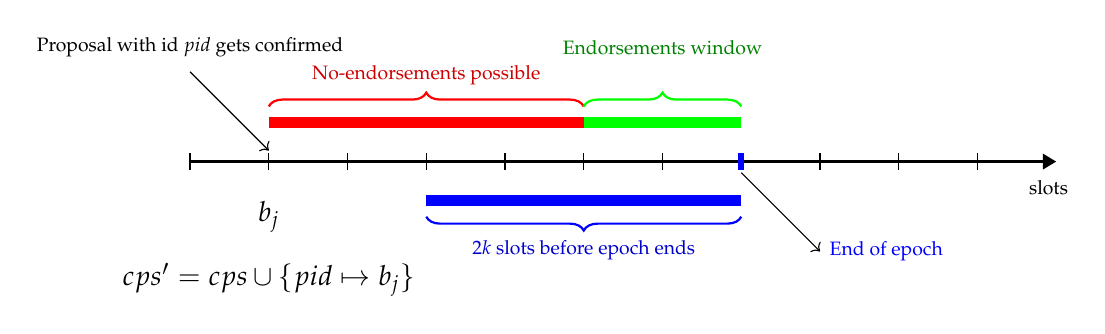
\begin{tikzpicture}
    %%
    %% Macros used in this picture
    %%
    %
    % Number of slots
    \pgfmathsetmacro{\nrSlots}{11}
    % Slot in which the proposal gets confirmed
    \pgfmathsetmacro{\cSlot}{1}
    % Our special K.
    \pgfmathsetmacro{\K}{2}
    % Epoch end.
    \pgfmathsetmacro{\eend}{7}

    % Draw the horizontal line
    \draw[thick, -Triangle] (0,0) -- (\nrSlots,0)
    node[font=\scriptsize,below left=3pt and -8pt]{slots};

    % % draw vertical lines
    \foreach \x in {0,1,...,10}
    \draw (\x cm, 3pt) -- (\x cm, -3pt);

    % Add a label to with the block number in which the proposal got confirmed.
    \node at (\cSlot, -.7) {$b_j$};

    % Update in cps
    \node at (\cSlot, -1.5) {$\var{cps'} = \var{cps} \cup \{ \var{pid} \mapsto b_j \}$};

    % The no-endorsements red bar.
    \draw[red, line width=4pt] (\cSlot, .5) -- +(2*\K, 0);

    % Brace above the no-endorsement window bar.
    \draw[thick, red, decorate, decoration={brace, amplitude=5pt}]
    (\cSlot, .7) -- +(2*\K, 0)
    node[black!20!red, midway, above=4pt, font=\scriptsize] {No-endorsements possible};

    % The endorsements window.
    \coordinate (ewStart) at (\cSlot + 2*\K, .5);
    \coordinate (ewEnd) at ($(\eend, .5)$);
    \draw[green, line width=4pt]
    (ewStart) -- (ewEnd);

    % Brace above the endorsements window
    \coordinate (ewStartB) at ($(ewStart) + (0, 0.2)$);
    \coordinate (ewEndB) at ($(ewEnd) + (0, 0.2)$);
    \draw[thick, green, decorate, decoration={brace, amplitude=5pt}]
    (ewStartB) -- (ewEndB)
    node[black!50!green, midway, above=15pt, font=\scriptsize] {Endorsements window};

    % The 2k before end-of-epoch window.
    \coordinate (beeStart) at (\eend - 2*\K, -.5);
    \coordinate (beeEnd) at ($(\eend, -.5)$);
    \draw[blue, line width=4pt]
    (beeStart) -- (beeEnd);

    % Brace on above the 2k before end-of-epoch window.
    \coordinate (beeStartB) at ($(beeStart) - (0, 0.2)$);
    \coordinate (beeEndB) at ($(beeEnd) - (0, 0.2)$);
    \draw[thick, blue, decorate, decoration={brace, amplitude=5pt}]
    (beeEndB) -- (beeStartB)
    node[black!20!blue, midway, below=5pt, font=\scriptsize] {$2k$ slots before epoch ends};

    \draw[blue, line width=2pt] (\eend, 3pt) -- (\eend, -3pt);

    \draw[<-] (\cSlot, 4pt) -- +(-1, 1)
    node [above=2pt, black, font=\scriptsize]
    {Proposal with id $\var{pid}$ gets confirmed};

    \draw[->] (\eend, -4pt) -- +(1, -1)
    node[right, blue, font=\scriptsize] {End of epoch};
  \end{tikzpicture}
  \caption{An update proposal confirmed too late}
  \label{fig:up-confirmed-too-late}
\end{figure}

\clearpage

\subsection{Deviations from the actual implementation}
\label{sec:deviation-actual-impl}

The current specification of the voting mechanism deviates from the actual
implementation, although it should be backwards compatible with the latter.
These deviations are required to simplify the voting and update mechanism
removing unnecessary features for a simplified setting, which will use the OBFT
consensus protocol with federated genesis key holders. This in turn, enables us
to remove any accidental complexity that might have been introduced in the
current implementation. The following subsections highlight the differences
between the this specification and the current implementation.

\subsubsection{Positive votes}
\label{sec:only-positive-votes}

Genesis keys can only vote (positively) for an update proposal. In the current
implementation stakeholders can vote for or against a proposal, which makes the
voting logic more complex:
\begin{itemize}
\item there are more cases to consider
\item the current voting validation rules allow voters to change their minds
  (by flipping their vote) at most once, which requires to keep track how a
  stake holder voted and how many times. Contrast this with
  Rule~\ref{eq:rule:voting} where we only need to keep track of the set of
  key-proposal-id's pairs.
\end{itemize}

\subsubsection{Alternative version numbers}
\label{sec:alt-version-numbers-constraints}

Alternative version numbers are only lexicographically constrained. The current
implementation seems to be dependent on the order in which the update proposals
arrive: given a new update proposal $\var{up}$, if a set $X$ of update
proposals with the same minor and major versions than $\var{up}$ exist, then
the alternative version of $\var{up}$ has to be one more than the maximum
alternative number of $X$. Not only this logic seems to be brittle since it
depends on the order of arrival of the update proposals, but it requires a more
complex check (which depends on state) to determine if a proposed version can
follow the current one. By being more lenient on the alternative versions of
update proposals we can simplify the version checking logic considerably.

\subsubsection{No implicit agreement}
\label{sec:no-implicit-agreement}

We do not model the implicit agreement rule. If a proposal does not get enough
votes before the end of the voting period, then we simply discard it. At the
moment it is not clear whether the implicit agreement rule is needed.

\subsubsection{Adoption threshold}
\label{sec:adoption-threshold}

The current implementation adopts a proposal with version $\var{pv}$ if the
portion of block issuers' stakes, which issued blocks with this version, is
greater than the threshold given by:

\begin{lstlisting}
max spMinThd (spInitThd - (t - s) * spThdDecrement)
\end{lstlisting}

where:
\begin{itemize}
\item \lstinline{spMinThd} is a minimum threshold required for adoption.
\item \lstinline{spInitThd} is an initial threshold.
\item \lstinline{spThdDecrement} is the decrement constant of the initial
  threshold.
\end{itemize}

In this specification we only make use of a minimum adoption threshold,
represented by the protocol parameter $\var{upAdptThd}$ until it becomes clear
why a dynamic alternative is needed.

\subsubsection{No checks on unlock-stake-epoch parameter}
\label{sec:no-unlock-stake-epoch-check}

The rule of Figure~\ref{eq:rule:up-validity} does not check the
\lstinline{bvdUnlockStakeEpoch} parameter, since it will have a different
meaning in the handover phase: its use will be reserved for unlocking the
Ouroboros-BFT logic in the software.

\subsubsection{No grouping of proposals per-application name}
\label{sec:no-app-up-grouping}

It is unclear at this moment whether we need to model the applications names
and versions, so this aspect is not modeled in the present rules.

\subsubsection{Ignored attributes of proposals}

In Figure~\ref{fig:defs:update-proposals} the types
$\type{UpdData}$, and $\type{UpdAttrs}$ are only needed to model the fact that
an update proposal must sign such data, however, we do not use them for any
other purpose in this formalization.

\subsection{Questions}
\label{sec:up-questions}

This temporary section contains unanswered questions about the formalization of
update mechanism:

\begin{itemize}
\item Do we need to model the $\var{scriptVersion}$?
\end{itemize}


\section{Blockchain interface}
\label{sec:blockchain-interface}

\newcommand{\DIEnv}{\type{DIEnv}}
\newcommand{\DIState}{\type{DIState}}

\newcommand{\UPIEnv}{\type{UPIEnv}}
\newcommand{\UPIState}{\type{UPIState}}

\subsection{Delegation interface}
\label{sec:delegation-interface}

\begin{figure}[htb]
  \emph{Delegation interface environments}
  \begin{equation*}
    \DIEnv =
    \left(
      \begin{array}{r@{~\in~}lr}
        \mathcal{K} & \powerset{\VKeyGen} & \text{allowed delegators}\\
        \var{e} & \Epoch & \text{epoch}\\
        \var{s} & \Slot & \text{slot}\\
        \var{d} & \SlotCount & \text{certificate liveness parameter}
      \end{array}
    \right)
  \end{equation*}

  \emph{Delegation interface states}
  \begin{equation*}
    \DIState
    = \left(
      \begin{array}{r@{~\in~}lr}
        \var{dms} & \VKeyGen \mapsto \VKey & \text{delegation map}\\
        \var{dws} & \VKeyGen \mapsto \Slot & \text{when last delegation occurred}\\
        \var{sds} & \seqof{(\Slot \times (\VKeyGen \times \VKey))} & \text{scheduled delegations}\\
        \var{eks} & \powerset{(\Epoch \times \VKeyGen)} & \text{key-epoch delegations}
      \end{array}
    \right)
  \end{equation*}

  \emph{Delegation transitions}
  \begin{equation*}
    \_ \vdash \_ \trans{deleg}{\_} \_ \in
    \powerset (\DIEnv \times \DIState \times \seqof{\DCert} \times \DIState)
  \end{equation*}
  \caption{Delegation interface transition-system types}
  \label{fig:ts-types:delegation-interface}
\end{figure}

\subsubsection{Delegation interface rules}
\label{sec:delegation-interface-rules}

\begin{figure}[htb]
  \begin{equation}
    \label{eq:rule:delegation-interface}
    \inference
    {
      {\begin{array}{l}
         \mathcal{K} \\
         e\\
         s\\
         d
       \end{array}}
      \vdash
      {
        \left(
          \begin{array}{l}
            \var{sds}\\
            \var{eks}
          \end{array}
        \right)
      }
      \trans{sdelegs}{\Gamma}
      {
        \left(
          \begin{array}{l}
            \var{sds'}\\
            \var{eks'}
          \end{array}
        \right)
      }
      &
      {
        \left(
          \begin{array}{l}
            \var{dms}\\
            \var{dws}
          \end{array}
        \right)
      }
      \trans{adelegs}{[.., s] \restrictdom \var{sds'}}
      {
        \left(
          \begin{array}{l}
            \var{dms'}\\
            \var{dws'}
          \end{array}
        \right)
      }
    }
    {
      {\begin{array}{l}
         \mathcal{K} \\
         e\\
         s\\
         d
      \end{array}}
      \vdash
      {
        \left(
          \begin{array}{l}
            \var{dms}\\
            \var{dws}\\
            \var{sds}\\
            \var{eks}
          \end{array}
        \right)
      }
      \trans{deleg}{\Gamma}
      {
        \left(
          \begin{array}{l}
            \var{dms'}\\
            \var{dws'}\\
            \var{[s-d,~ s+d]} \restrictdom \var{sds'}\\
            \var{[e, ..]} \restrictdom \var{eks'}
          \end{array}
        \right)
      }
    }
  \end{equation}
  \caption{Delegation interface rules}
  \label{fig:rules:delegation-interface}
\end{figure}

\subsubsection{Delegation interface functions}
\label{sec:delegation-interface-functions}

\begin{figure}[htb]
  \begin{align*}
    & \fun{delegates} \in \DIState \to (\VKeyGen \times \VKey) \to \Bool & \text{delegation relationship}\\
    & \fun{delegates}~s~(\var{vk_s}, \var{vk_d}) = \var{vk_s} \mapsto \var{vk_d} \in (\var{dms}~s)\\
    \nextdef
    & \fun{initialDS} \in \VKeyGen \to \DIState & \text{initial delegation state}\\
    & \fun{initialDS}~\var{ks} =
      \left(
      \begin{array}{l}
        \var{ks} \mapsto \var{ks}\\
        \emptyset\\
        \epsilon\\
        \emptyset\\
      \end{array}
      \right)
  \end{align*}
  \caption{Delegation interface functions}
\end{figure}

\clearpage

\subsection{Update-proposals interface}
\label{sec:update-proposals-interface}

Figure~\ref{fig:ts-types:upi} defines the types of the transition systems
related with the update-proposals interface. The acronyms in the transition
labels have the following meaning:
\begin{description}
\item[UPIREG] Update-proposal-interface registration.
\item[UPIVOTE] Update-proposal-interface vote.
\item[UPIEND] Update-proposal-interface endorsement.
\item[UPIEC] Update-proposal-interface epoch-change.
\end{description}

\begin{figure}[htb]
  \emph{Update-proposals interface environments}
  \begin{align*}
    & \UPIEnv
      = \left(
      \begin{array}{r@{~\in~}lr}
        \var{k} & \mathbb{N} & \text{chain stability parameter}\\
        \var{u} & \mathbb{N} & \text{update proposals time-to-live}\\
        \var{e_c} & \Epoch & \text{current epoch}\\
        \var{b_n} & \BkNr & \text{current block number}\\
        \var{dms} & \VKeyGen \mapsto \VKey & \text{delegation map}\\
      \end{array}\right)
  \end{align*}
  %
  \emph{Update-proposals interface states}
  \begin{align*}
    & \UPIState = \\
    & \left(
      \begin{array}{r@{~\in~}lr}
        \var{e_p} & \Epoch & \text{previously seen epoch}\\
        (\var{pv}, \var{pps}) & \ProtVer \times \PPMMap
        & \text{current protocol information}\\
        (\var{pv_c}, \var{pps_c}) & \ProtVer \times \PPMMap
        & \text{candidate protocol information}\\
        \var{avs} & \ApName \mapsto (\mathbb{N} \times \BkNr)
        & \text{application versions}\\
        \var{rups} & \UPropId \mapsto (\ProtVer \times \PPMMap)
        & \text{registered protocol update proposals}\\
        \var{raus} & \UPropId \mapsto (\ApName \times \mathbb{N})
        & \text{registered software update proposals}\\
        \var{eps} & \powerset{(\Epoch \times \VKeyGen)}
        & \text{proposals per-epoch per-key}\\
        \var{cps} & \UPropId \mapsto \BkNr & \text{confirmed proposals}\\
        \var{vts} & \powerset{(\UPropId \times \VKeyGen)} & \text{proposals votes}\\
        \var{bvs} & \powerset{(\ProtVer \times \VKeyGen)}
                           & \text{endorsement-key pairs}\\
        \var{pws} & \UPropId \mapsto \BkNr & \text{proposal timestamps}
      \end{array}\right)\\
  \end{align*}
  %
  \emph{Update-proposals interface transitions}
  \begin{equation*}
    \begin{array}{r@{~\in~}l}
      \_ \vdash \_ \trans{upireg}{\_} \_ &
      \powerset (\UPIEnv \times \UPIState \times \UProp \times \UPIState)\\
      \_ \vdash \_ \trans{upivote}{\_} \_ &
      \powerset (\UPIEnv \times \UPIState \times \Vote \times \UPIState)\\
      \_ \vdash \_ \trans{upiend}{\_} \_ &
      \powerset (\UPIEnv \times \UPIState
      \times (\ProtVer \times \VKey) \times \UPIState)\\
      \_ \vdash \_ \trans{upiec}{\_} \_ &
      \powerset (\UPIEnv \times \UPIState \times \Epoch \times \UPIState)
    \end{array}
  \end{equation*}
  \caption{Update-proposals interface transition-system types}
  \label{fig:ts-types:upi}
\end{figure}

\begin{figure}[htb]
  \begin{equation}
    \label{eq:rule:upi-reg-interface}
    \inference
    {
      {
        \begin{array}{l}
          \var{pv}\\
          \var{pps}\\
          \var{e_c}\\
          \var{avs}\\
          \var{dms}
        \end{array}
      }
      \vdash
      {
        \left(
          \begin{array}{l}
            \var{rups}\\
            \var{raus}\\
            \var{eps}
          \end{array}
        \right)
      }
      \trans{upreg}{\var{up}}
      {
        \left(
          \begin{array}{l}
            \var{rups'}\\
            \var{raus'}\\
            \var{eps'}
          \end{array}
        \right)
      }
      &
      pws' = pws \unionoverride \{ \upId{up} \mapsto b_n\}
    }
    {
      {
        \begin{array}{l}
          k\\
          u\\
          e_c\\
          b_n\\
          \var{dms}
        \end{array}
      }
      \vdash
      {
        \left(
          \begin{array}{l}
            \var{e_p}\\
            (\var{pv}, \var{pps})\\
            (\var{pv_c}, \var{pps_c})\\
            \var{avs}\\
            \var{rups}\\
            \var{raus}\\
            \var{eps}\\
            \var{cps}\\
            \var{vts}\\
            \var{bvs}\\
            \var{pws}
          \end{array}
        \right)
      }
      \trans{upireg}{\var{up}}
      {
        \left(
          \begin{array}{l}
            \var{e_p}\\
            (\var{pv}, \var{pps})\\
            (\var{pv_c}, \var{pps_c})\\
            \var{avs}\\
            \var{rups'}\\
            \var{raus'}\\
            \var{eps'}\\
            \var{cps}\\
            \var{vts}\\
            \var{bvs}\\
            \var{pws'}
          \end{array}
        \right)
      }
    }
  \end{equation}
  \caption{Update-proposals registration rules}
  \label{fig:rules:upi-reg-interface}
\end{figure}

\clearpage

Rule~\ref{eq:rule:upi-vote} models the effect of voting on an update proposal:
after a vote, a proposal might get confirmed, which means that it will be added
to the set $\var{cps'}$. In such case, the mapping of application names to
their latest version known to the ledger will be updated to include the
information in the confirmed proposal. Note that, unlike protocol updates,
software updates take effect as soon as a proposal is confirmed. In this rule,
we also delete the confirmed proposal id's from the set of registered
application update proposals ($\var{raus}$), since this information is no
longer needed once the application-name to software-version map ($\var{avs}$) is
updated.

\begin{figure}[htb]
  \begin{equation}
    \label{eq:rule:upi-vote}
    \inference
    {
      {
        \begin{array}{l}
          b_n\\
          \var{pps}\\
          \var{rups}\\
          \var{dms}
        \end{array}
      }
      \vdash
      {
        \left(
          \begin{array}{l}
            \var{cps}\\
            \var{vts}
          \end{array}
        \right)
      }
      \trans{upvote}{\var{v}}
      {
        \left(
          \begin{array}{l}
            \var{cps'}\\
            \var{vts'}
          \end{array}
        \right)
      }\\
      \var{avs_{new}} = \{ \var{an} \mapsto (\var{av}, \var{b_n})
      \mid \var{pid} \mapsto (\var{an}, \var{av}) \in \var{raus}
      ,~ \var{pid} \in \dom~\var{cps'}
      \}
    }
    {
      {
        \begin{array}{l}
          k\\
          u\\
          e_c\\
          b_n\\
          \var{dms}
        \end{array}
      }
      \vdash
      {
        \left(
          \begin{array}{l}
            \var{e_p}\\
            (\var{pv}, \var{pps})\\
            (\var{pv_c}, \var{pps_c})\\
            \var{avs}\\
            \var{rups}\\
            \var{raus}\\
            \var{eps}\\
            \var{cps}\\
            \var{vts}\\
            \var{bvs}\\
            \var{pws}
          \end{array}
        \right)
      }
      \trans{upivote}{\var{v}}
      {
        \left(
          \begin{array}{l}
            \var{e_p}\\
            (\var{pv}, \var{pps})\\
            (\var{pv_c}, \var{pps_c})\\
            \var{avs} \unionoverride \var{avs_{new}}\\
            \var{rups}\\
            \dom~ \var{cps} \subtractdom \var{raus}\\
            \var{eps}\\
            \var{cps'}\\
            \var{vts'}\\
            \var{bvs}\\
            \var{pws}
          \end{array}
        \right)
      }
    }
  \end{equation}
  \caption{Voting on update-proposals rules}
  \label{fig:rules:upi-vote}
\end{figure}

Figure~\ref{fig:st-diagram-sw-up} shows the different states in which a
software proposal update might be: if valid, a software update proposal becomes
active whenever it is included in a block. If the update proposal gets enough
votes, then the corresponding software update proposal becomes confirmed, and
the ledger state reflects this. If the voting period ends without an update
proposal being confirmed, then the corresponding software update proposal gets
rejected.
%
Protocol updates on the other hand, involve a slightly different logic, and the
state transition diagram for these kind of updates is shown in
Figure~\ref{fig:st-diagram-pt-up}.

\begin{figure}[ht]
  \centering
  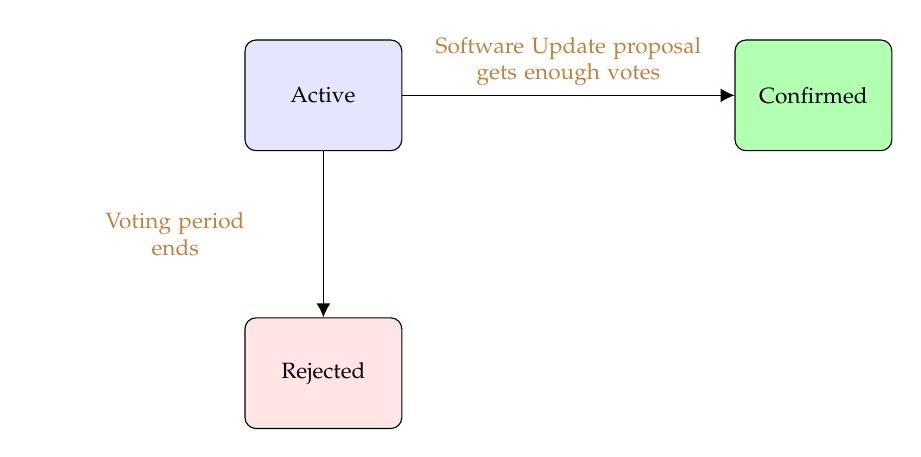
\begin{tikzpicture}[ align = center
                     , node distance = 6em and 12em
                     , text width = 5em
                     , font = \footnotesize
                     , >={Latex[width=0.5em, length=0.5em]}
                     , every node/.style = { rectangle
                                         , rounded corners
                                         , draw = black
                                         , align = center
                                         , minimum height = 4em }
                     ]

  \node (active) [fill = blue!10] {Active};
  \node (rejected) [below = of active, fill = red!10] {Rejected};
  \node (confirmed) [right = of active, fill = green!30] {Confirmed};

  \tikzset{every node/.style={align=center, text width=10em, text=brown}}

  \draw[->] (active)
  edge node [above] {Software Update proposal\\ gets enough votes}
  (confirmed);

  \draw[->] (active)
  edge node [left] {Voting period \\ends}
  (rejected);

  \end{tikzpicture}

  \caption{State-transition diagram for software-updates}
  \label{fig:st-diagram-sw-up}
\end{figure}

\clearpage

The interface rule for protocol-version endorsement makes use of the
$\trans{upend}{}$ transition, passing only the portion of the state relevant
to it. In addition, the unconfirmed proposals that are older than $u$ blocks
are removed from the parts of the state that hold:
\begin{itemize}
\item the registered protocol and software update proposals,
\item the votes associated with the proposals,
\item the set of endorsement-key pairs, and
\item the block number in which proposals where added.
\end{itemize}
The epoch-key pairs set ($\var{eps}$) that represents which stakeholder
proposed an update in which epoch, is cleaned up in the rules given in
\cref{fig:rules:upi-ec}, which deals with epoch change.

In Rule~\ref{eq:rule:upi-pend}, the set of proposal id's $\var{pid_{keep}}$
contains only those proposals that haven't expired yet or that are confirmed.
Once a proposal $\var{up}$ is confirmed, it is removed from the set of
confirmed proposals ($\var{cps}$) either when it is adopted or when a protocol
version higher than that of $\var{up}$ gets adopted (see
Rule~\ref{eq:rule:upi-ec}).
%
The set of endorsement-key pairs is cleaned here as well as in the epoch change
rule (Rule~\ref{eq:rule:upi-ec}). The reason for this is that this set grows at
each block, and it can get considerably large if no proposal gets adopted at
the end on an epoch.

\begin{figure}[htb]
  \begin{equation}
    \label{eq:rule:upi-pend}
    \inference
    {
      {
        \begin{array}{l}
          k\\
          b_n\\
          (\var{pv}, \var{pps})\\
          \var{dms}\\
          \var{cps}\\
          \var{rups}
        \end{array}
      }
      \vdash
      {
        \left(
          \begin{array}{l}
            (\var{pv_c}, \var{pps_c})\\
            \var{bvs}
          \end{array}
        \right)
      }
      \trans{upend}{(\var{bv}, \var{vk})}
      {
        \left(
          \begin{array}{l}
            (\var{pv_c'}, \var{pps_c'})\\
            \var{bvs'}
          \end{array}
        \right)
      }\\
      {
        \begin{array}{r@{~=~}l}
          \var{pids_{keep}} & \dom~(pws \restrictrange [b_n - u, ..]) \cup \dom~\var{cps}\\
          \var{vs_{keep}} & \dom~(\range~\var{rups'})\\
          \var{rups'} & \var{pids_{keep}} \restrictdom \var{rups}
        \end{array}
      }
    }
    {
      {
        \begin{array}{l}
          k\\
          u\\
          e_c\\
          b_n\\
          \var{dms}
        \end{array}
      }
      \vdash
      {
        \left(
          \begin{array}{l}
            \var{e_p}\\
            (\var{pv}, \var{pps})\\
            (\var{pv_c}, \var{pps_c})\\
            \var{avs}\\
            \var{rups}\\
            \var{raus}\\
            \var{eps}\\
            \var{cps}\\
            \var{vts}\\
            \var{bvs}\\
            \var{pws}
          \end{array}
        \right)
      }
      \trans{upiend}{(\var{bv}, \var{vk})}
      {
        \left(
          \begin{array}{l}
            \var{e_p}\\
            (\var{pv}, \var{pps})\\
            (\var{pv_c'}, \var{pps_c'})\\
            \var{avs}\\
            \var{rups'}\\
            \var{pids_{keep}} \restrictdom \var{raus}\\
            \var{eps}\\
            \var{cps}\\
            \var{pids_{keep}} \restrictdom \var{vts}\\
            \var{vs_{keep}}  \restrictdom \var{bvs}\\
            \var{pids_{keep}} \restrictdom \var{pws}
          \end{array}
        \right)
      }
    }
  \end{equation}
  \caption{Proposal endorsement rules}
  \label{fig:rules:upi-pend}
\end{figure}

\clearpage

Rule~\ref{eq:rule:upi-ec} models how the protocol version and its parameters
are changed depending on the epoch in the signal ($e_n$ in this case). A change
only occurs if the new epoch is greater than the previously seen epoch ($e_p$).
In such case, the current epoch is also updated accordingly. The candidate
versions and parameters map $(\var{pv_c}, \var{pps_c})$ remain constant in this
transition, even if they become adopted. Note that, in the final state, we use
union override to define the updated parameters
($\var{pps} \unionoverride \var{pps'}$). This is because candidate proposal
might only update some parameters of the protocol.

Rule~\ref{eq:rule:upi-ec} performs cleanup of several state variables:
\begin{itemize}
\item We keep only the information of proposals whose proposed
  protocol-versions are greater than the newly adopted protocol version
  ($\var{pv'}$). This means that active proposals will be discarded even if the
  voting period is not over (it makes no sense to vote on a proposal that
  proposes to upgrade to an older version of the protocol).
\item The set $\var{eps}$ is updated so that only keys that proposed in epochs
  no earlier than $e_n$ are kept.
\item The registered software-update proposals need not be cleaned here, since
  this is done either when a proposal gets confirmed or when it expires.
\end{itemize}

\begin{figure}[htb]
  \begin{equation}
    \label{eq:rule:pvbump-change-noop}
    \inference
    {
      e_n \leq e_p
    }
    {
      (\var{pv_c}, \var{pps_c})
      \vdash
      {
        \left(
          \begin{array}{l}
            \var{e_p}\\
            \var{(\var{pv}, \var{pps})}\\
          \end{array}
        \right)
      }
      \trans{pvbump}{\var{e_n}}
      {
        \left(
          \begin{array}{l}
            \var{e_p}\\
            \var{(\var{pv}, \var{pps})}\\
          \end{array}
        \right)
      }
    }
  \end{equation}
  \nextdef
  \begin{equation}
    \label{eq:rule:pvbump-change}
    \inference
    {
      e_p < e_n
    }
    {
      (\var{pv_c}, \var{pps_c})
      \vdash
      {
        \left(
          \begin{array}{l}
            \var{e_p}\\
            \var{(\var{pv}, \var{pps})}
          \end{array}
        \right)
      }
      \trans{pvbump}{\var{e_n}}
      {
        \left(
          \begin{array}{l}
            \var{e_n}\\
            \var{(\var{pv_c}, \var{pps_c})}
          \end{array}
        \right)
      }
    }
  \end{equation}
  \nextdef
  \begin{equation}
    \label{eq:rule:upi-ec}
    \inference
    {
      (\var{pv_c}, \var{pps_c})
      \vdash
      {
        \left(
          \begin{array}{l}
            \var{e_p}\\
            \var{(\var{pv}, \var{pps})}
          \end{array}
        \right)
      }
      \trans{pvbump}{\var{e_n}}
      {
        \left(
          \begin{array}{l}
            \var{e'}\\
            \var{(\var{pv'}, \var{pps'})}\\
          \end{array}
        \right)
      }\\ ~ \\
      \var{pids_{keep}} = \{ \var{pid} \mid
      \var{pid} \mapsto (\var{pv_i}, \wcard) \in \var{rups}
      ,~ \var{pv'} \leq \var{pv_i}\}
    }
    {
      {
        \begin{array}{l}
          k\\
          u\\
          e_c\\
          b_n\\
          \var{dms}\\
        \end{array}
      }
      \vdash
      {
        \left(
          \begin{array}{l}
            \var{e_p}\\
            \var{(\var{pv}, \var{pps})}\\
            \var{(\var{pv_c}, \var{pps_c})}\\
            \var{avs}\\
            \var{rups}\\
            \var{raus}\\
            \var{eps}\\
            \var{cps}\\
            \var{vts}\\
            \var{bvs}\\
            \var{pws}
          \end{array}
        \right)
      }
      \trans{upiec}{\var{e_n}}
      {
        \left(
          \begin{array}{l}
            \var{e'}\\
            \var{(\var{pv'}, \var{pps} \unionoverride \var{pps'})}\\
            \var{(\var{pv_c}, \var{pps_c})}\\
            \var{avs}\\
            \var{pids_{keep}} \restrictdom \var{rups}\\
            \var{raus}\\
            {[e_n, ..]} \restrictdom \var{eps}\\
            \var{pids_{keep}} \restrictdom \var{cps}\\
            \var{pids_{keep}} \restrictdom \var{vts}\\
            {[\var{pv'}, ..]} \restrictdom \var{bvs}\\
            \var{pids_{keep}} \restrictdom \var{pws}
          \end{array}
        \right)
      }
    }
  \end{equation}
  \caption{Block version adoption on epoch change rules}
  \label{fig:rules:upi-ec}
\end{figure}

Figure~\ref{fig:st-diagram-pt-up} shows the different states a protocol-update
proposal can be in, and what causes the transitions between them.

\begin{figure}[ht]
  \centering
  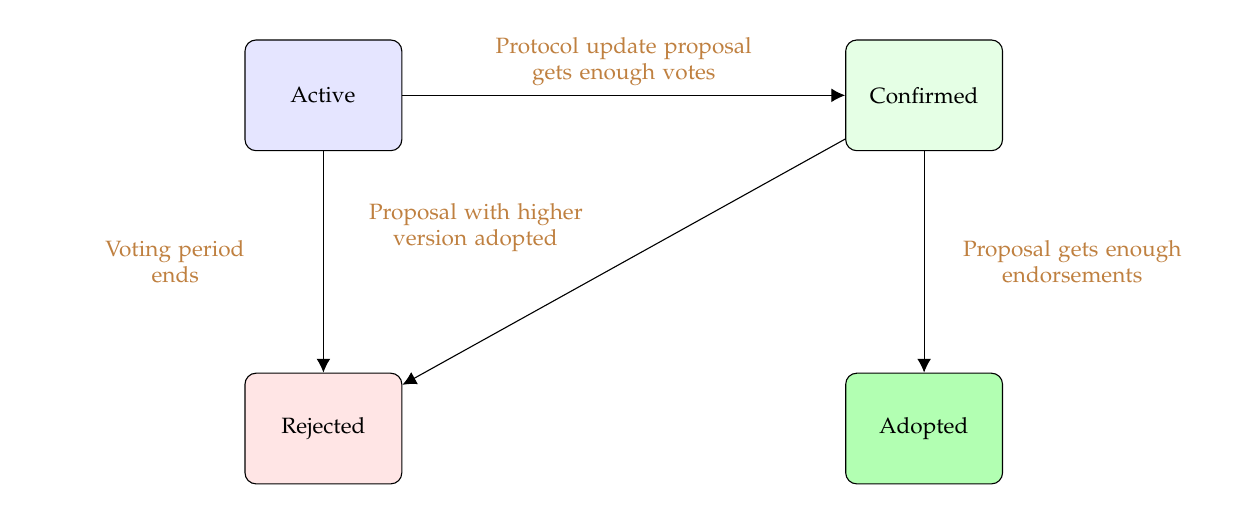
\begin{tikzpicture}[ align = center
                     , node distance = 8em and 16em
                     , text width = 5em
                     , font = \footnotesize
                     , >={Latex[width=0.5em, length=0.5em]}
                     , every node/.style = { rectangle
                                         , rounded corners
                                         , draw = black
                                         , align = center
                                         , minimum height = 4em }
                     ]

  \node (active) [fill = blue!10] {Active};
  \node (rejected) [below = of active, fill = red!10] {Rejected};
  \node (confirmed) [right = of active, fill = green!10] {Confirmed};
  \node (adopted) [below = of confirmed, fill = green!30] {Adopted};

  \tikzset{every node/.style={align=center, text width=10em, text=brown}}

  \draw[->] (active)
  edge node [above] {Protocol update proposal\\ gets enough votes}
  (confirmed);

  \draw[->] (active)
  edge node [left] {Voting period \\ends}
  (rejected);

  \draw[->] (confirmed)
  edge node [above left]
  {Proposal with higher version adopted}
  (rejected);

  \draw[->] (confirmed)
  edge node [right]
  {Proposal gets enough endorsements}
  (adopted);

  \end{tikzpicture}

  \caption{State-transition diagram for protocol-updates}
  \label{fig:st-diagram-pt-up}
\end{figure}

\addcontentsline{toc}{section}{References}
\bibliographystyle{plainnat}
\bibliography{references}

\end{document}
